\documentclass[12pt]{article}

% \usepackage[utf8]{inputenc}
\usepackage[T1]{fontenc}
\usepackage[francais]{babel}
%Options: Sonny, Lenny, Glenn, Conny, Rejne, Bjarne, Bjornstrup
% \usepackage[Lenny]{fncychap}
% \usepackage{mathpazo}
\usepackage{fontspec}
\setmainfont[
    SmallCapsFont={TeX Gyre Termes},
    SmallCapsFeatures={Letters=SmallCaps},
]{ubuntu}
\usepackage[a4paper, width=150mm, top=25mm, bottom=25mm]{geometry}
\usepackage[colorlinks=true, linkcolor=blue, unicode]{hyperref}
\frenchbsetup{StandardLists=true}
\usepackage{enumitem}
\setlist[itemize]{label=\textbullet, topsep=0cm}
\setlist[description]{topsep=0cm}
\usepackage{parskip}
\usepackage{graphicx}
\usepackage{float}
\usepackage[bottom]{footmisc}
\usepackage[defaultlines=4,all]{nowidow}
\usepackage{subcaption}
\usepackage{array}

% To write inline code.
\usepackage{xcolor}
\definecolor{light-gray}{gray}{0.90}
\newcommand{\code}[1]{\colorbox{light-gray}{\texttt{#1}}}

\usepackage{listings}

\lstdefinestyle{code}{
language=python,
keywordstyle=\color{blue},
stringstyle=\color{red},
commentstyle=\color{gray},
basicstyle=\small\ttfamily,
numbers=left,
numberstyle=\normalsize,
numbersep=7pt,
showstringspaces=false,
breaklines=true,
frame=leftline,
framerule=2pt,
}

\lstdefinestyle{exec_result}{
frame=tb,
language=bash,
aboveskip=3mm,
belowskip=3mm,
showstringspaces=false,
columns=flexible,
basicstyle={\small\ttfamily},
numbers=none,
numberstyle=\tiny\color{gray},
breaklines=true,
breakatwhitespace=true,
framerule=2pt,
}

% To write texte in box. available boxes : notebox, tipbox, warningbox, cautionbox, importantbox, questionbox.
% How to use : questionbox{some texte here}.
\usepackage{awesomebox}
\def\abIconQuestion{\symbol{"F059}}
\newcommand{\questionbox}[1]{%
  \awesomebox{\abIconQuestion}{\aweboxrulewidth}{abwarning}{#1}}


\hyphenation{simp-le simp-les}


\title{Formation Python}
\author{Malaoui, Sidahmed Bilal}
\date{14 Février 2017}


\begin{document}
\pagenumbering{gobble}

\newcommand{\hsp}{\hspace{20pt}}
\newcommand{\HRule}{\rule{\linewidth}{0.5mm}}
\begin{titlepage}
  \begin{sffamily}
  \begin{center}

    % Upper part of the page. The '~' is needed because \\
    % only works if a paragraph has started.
    
\includegraphics[width=0.5\linewidth]{img/OMC_logo.png}~\\[1.5cm]

    \textsc{\LARGE Open Minds Club}\\[2cm]

    \textsc{\Large Formation}\\[1.5cm]

    % Title
    \HRule \\[0.4cm]
    { \huge \bfseries Langage Python\\[0.4cm] }

    \HRule \\[2cm]
    
\includegraphics[scale=0.2]{img/OMC_logo.png}
    \\[2cm]

    % Author and supervisor
    \begin{minipage}{0.4\textwidth}
      \begin{center} \large
        Sidahmed Bilal \textsc{Malaoui}\\
      \end{center}
    \end{minipage}

    \vfill

    % Bottom of the page
    {\large 14\iemes{} Février 2017 — 20 Mars 2017}

  \end{center}
  \end{sffamily}
\end{titlepage}

\clearpage
\renewcommand{\contentsname}{Sommaire}
\tableofcontents
\newpage

\pagenumbering{arabic}

\section{La programmation avec Python 3}
    \subsection{Introduction}
        Ceci est une petite introduction où on va parler des programmes et des langages de programmations.
        \subsubsection{C'est quoi un programme ??}
            Je vais commencer par donner une définition qui peut vous semblez un peu floue, mais cette description
            va s'éclaircir coûte que coûte au cours de notre formation.

            Alors, un programme est un ensemble d'instructions exécuté par l'ordinateur pour qu'il puisse (l'ordinateur)
            accomplir une tâche bien précise. On a pour exemple des programmes : les navigateurs web
            (comme chromium, chrome, firefox), qui permettent de visiter les sites et de chatter en ligne ;
            on a aussi les jeux vidéos, les logiciels de retouches de photos \ldots\ etc

            \begin{figure}[H]
                \centering
                \begin{subfigure}[b]{0.49\textwidth}
                    \centering
                    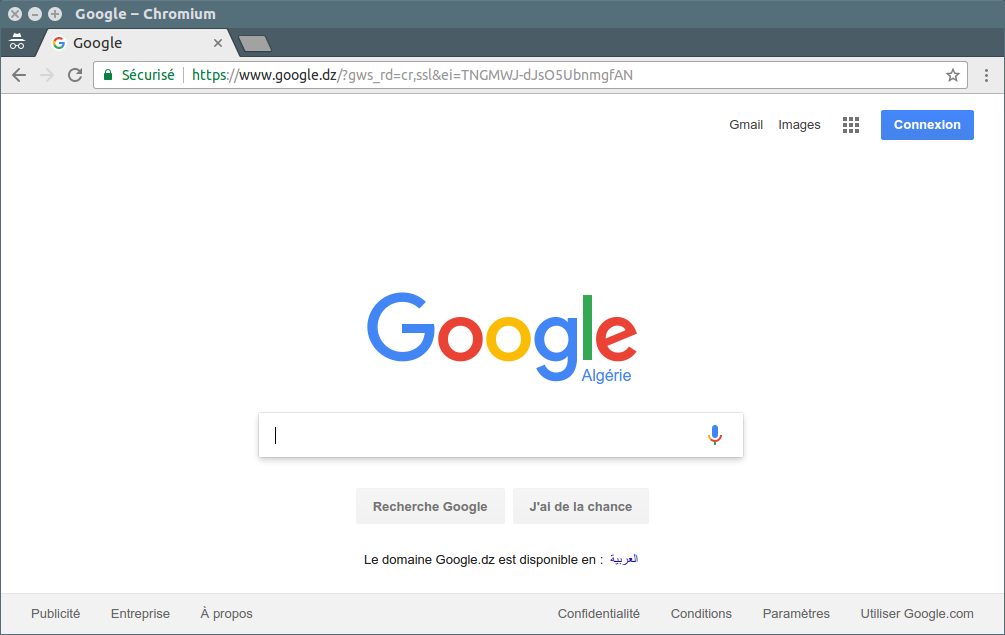
\includegraphics[width=\textwidth, height=2in]{img/1_chrome.png}
                    \caption{Google Chrome}
                \end{subfigure}
                \hfill
                \begin{subfigure}[b]{0.49\textwidth}
                    \centering
                    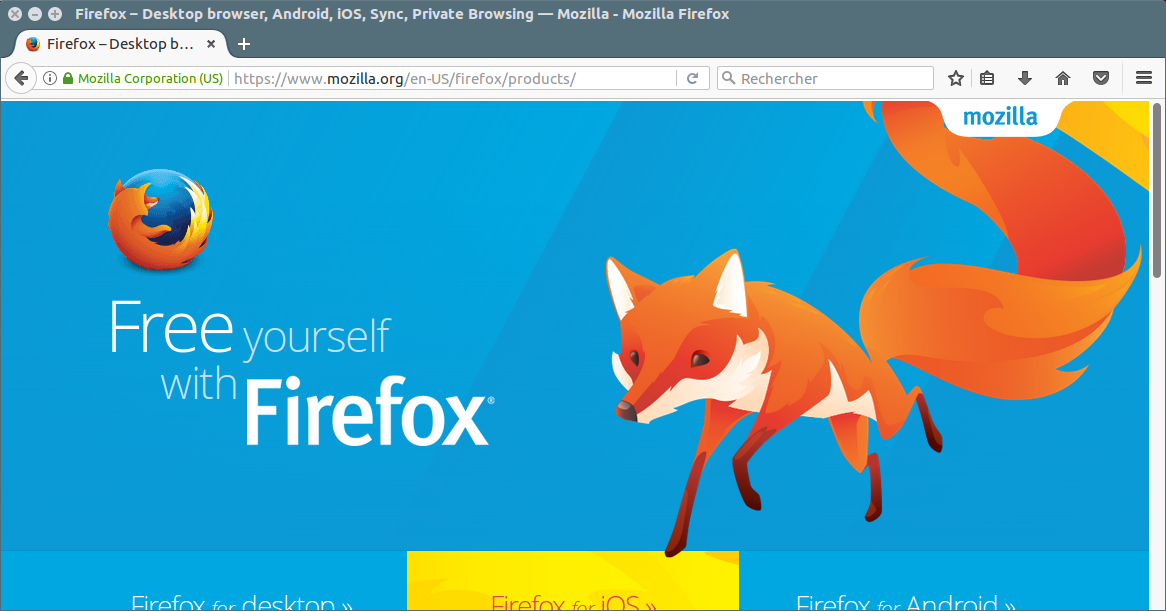
\includegraphics[width=\textwidth, height=2in]{img/2_firefox.png}
                    \caption{Mozilla Firefox}
                \end{subfigure}
            \end{figure}

            \begin{figure}[H]
                \centering
                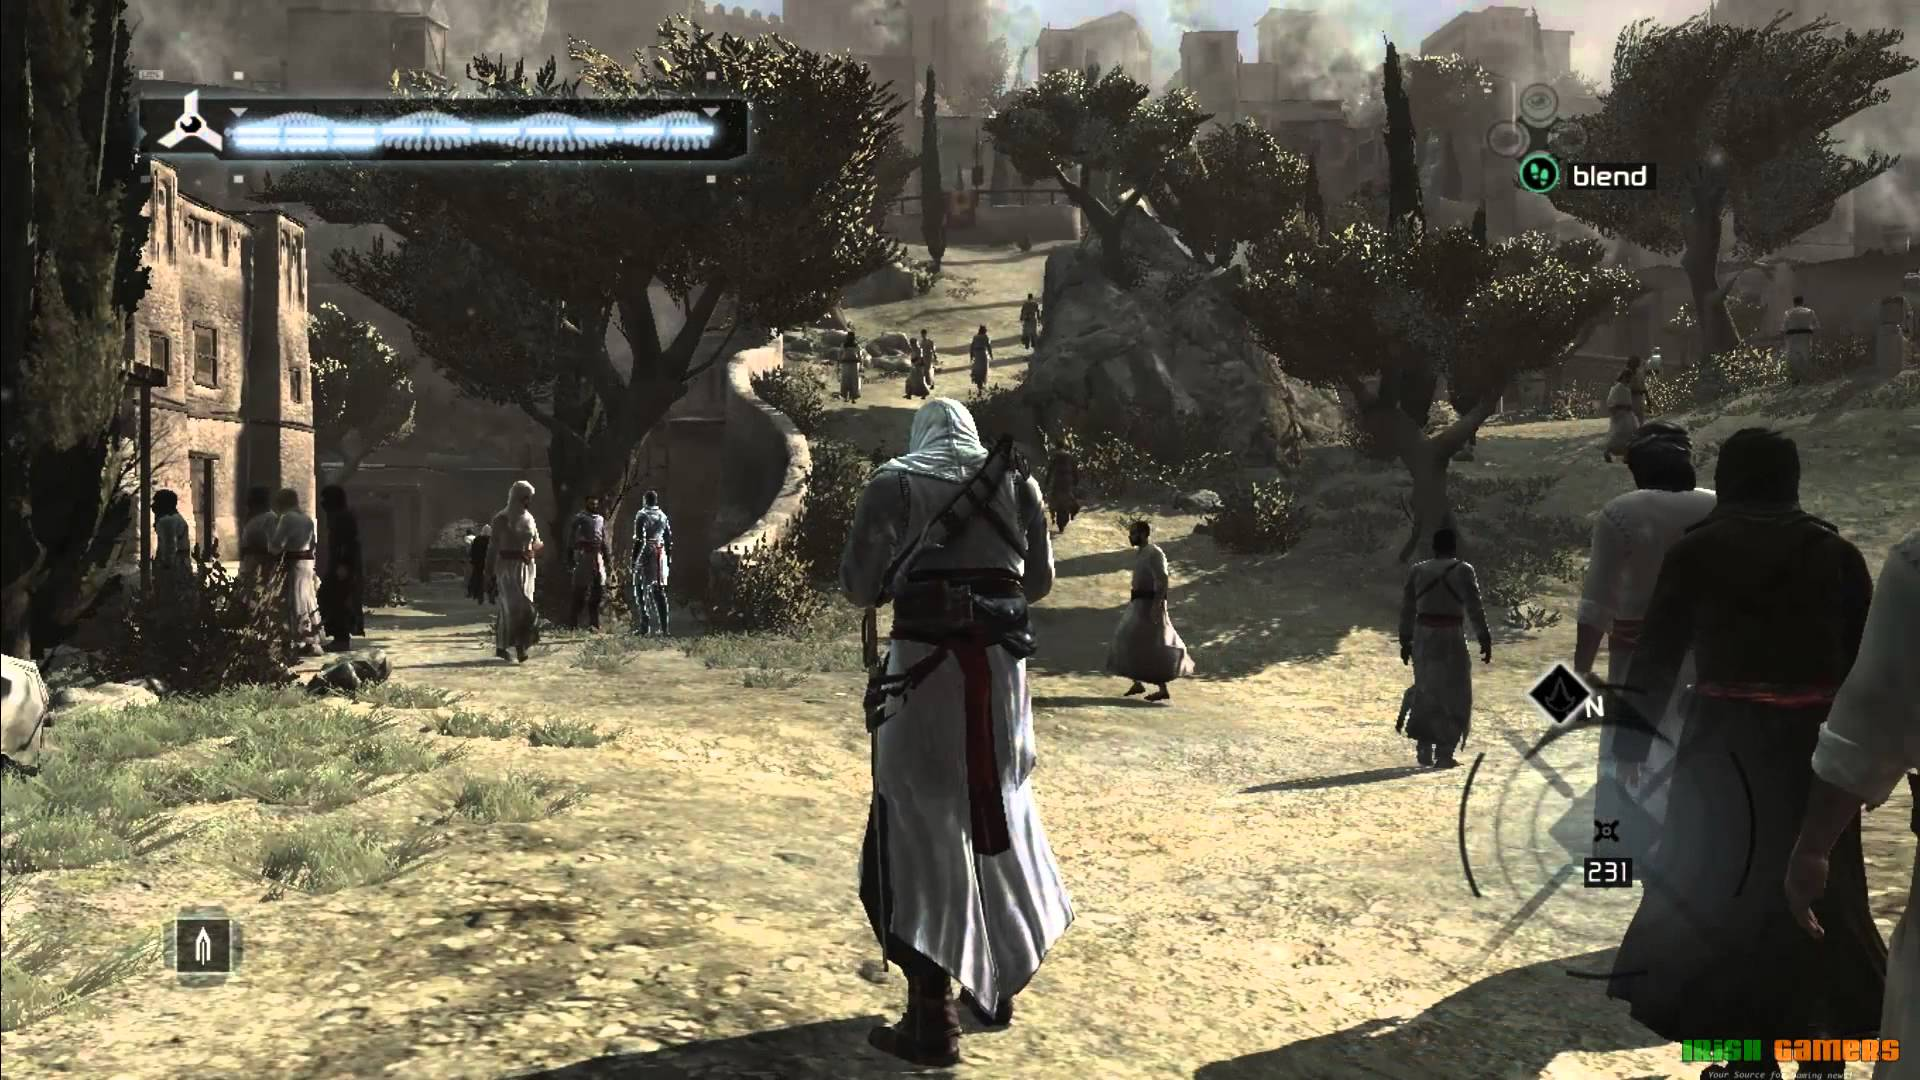
\includegraphics[width=\textwidth, height=2.5in]{img/3_assassins_creed.jpg}
                \caption{Le jeu Assassin's Creed}
            \end{figure}
            \begin{figure}[H]
                \centering
                
\includegraphics[width=\textwidth]{img/4_gimp.png}
                \caption{Logiciels de retouches ``Gimp''}
            \end{figure}
            % Dans tous les exemples citer avant, on voit que ces programme
            % demande à l'ordinateur d'exécuter des instructions pour qu'il puisse servir; tous ces programmes donnent des instructions bien précise à
            % l'ordinateur pour qu'il puisse accomplir certaines tâches

        \subsubsection{Comment sont crée ces programmes ??}
            L'ordinateur est une machine bête et discipliné qui ne comprend qu'un seul langage, qui est le langage
            \emph{binaire}. Ce langage est une succession de 1 et de 0 comme suit :
            \begin{lstlisting}[style=code,numbers=none]
01101100001100110011000111101011101
            \end{lstlisting}

            Donc, normalement, pour créer des programmes, il fallait apprendre ce langage.
            Mais heureusement, les informaticiens ont eu la réflexion de créer d'autres langages intermédiaires
            (qu'on appel langage de programmation) qui sont beaucoup plus facile que le binaire. Ces langage ont
            tous le même but : permettre de créer des programmes plus facilement qu'en binaire.

            Voici comment cela fonctionne :
            \begin{itemize}
                % \item On donne nos instructions à l'ordinateur en utilisant un langage de programmation.
                \item On écrit nos instructions en utilisant un langage de programmation.
                \item Les instructions sont traduites en binaire grâce à un programme de traduction.
                \item L'ordinateur peut alors lire le binaire et faire ce qu'on l'a demandé.
            \end{itemize}

            Voici une image qui illustre ce qu'on vient de dire :
            \begin{figure}[H]
                \centering
                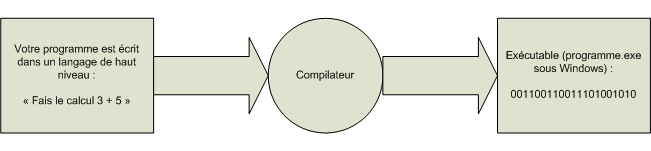
\includegraphics[width=\linewidth]{img/11_compilation.png}
                \caption{Les étapes de création d'un programme}
            \end{figure}

            \notebox{Une remarque très importante : les instructions que nous écrivons dans un langage de programmation
            sont appelé \textbf{Code Source}. Gardez bien ce terme à l'esprit, parce qu'on va beaucoup l'utiliser
            par la suite. Voici un exemple de code source python que nous écrirons plus tard :

            \begin{figure}[H]
                \centering
                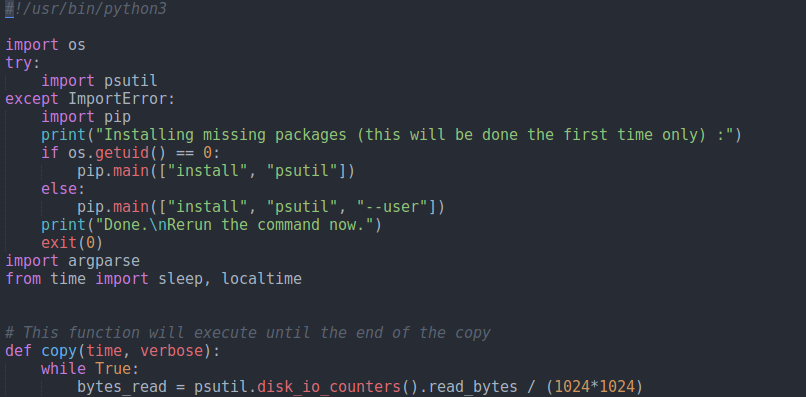
\includegraphics[width=\linewidth]{img/12_code.png}
                \caption{Coude source Python}
            \end{figure}
            }

        \subsubsection{Les langages de programmation les plus connus}
        \begin{figure}[H]
            \centering
            \begin{subfigure}[b]{0.32\textwidth}
                \centering
                
\includegraphics[width=\textwidth]{img/5_c++.png}
                \caption{Logo C++}
            \end{subfigure}
            \hfill
            \begin{subfigure}[b]{0.32\textwidth}
                \centering
                
\includegraphics[width=\textwidth]{img/6_java.png}
                \caption{Logo Java}
            \end{subfigure}
            \hfill
            \begin{subfigure}[b]{0.32\textwidth}
                \centering
                
\includegraphics[width=\textwidth]{img/7_python.png}
                \caption{Logo Python}
            \end{subfigure}
        \end{figure}

        \subsubsection{Compilé vs Interprété}
            Nous avons dit tout à l'heure que les instructions sont traduites en binaire pour que l'ordinateur puisse
            les comprendre et les exécuter. Mais ce qu'on a pas dit c'est qu'il y a deux façons de traduire
            les instructions : \emph{Compilation} et \emph{Interprétation}.

            \begin{description}
                \item[Compilation :] Avec ce processus, toutes nos instructions sont traduites en binaires à la fois.
                    Ce qui nous donne en résultat un gros fichier binaire qui peut être exécuté directement par
                    l'ordinateur.
                \item[Interprétation :] Avec cette technique, on ne traduit pas tous les instructions en binaires, mais
                    on va plutôt traduire une instruction par instruction à chaque fois qu'on veut exécuter
                    notre programme. Par exemple, si mon code source contient 3 instructions, quand je veux l'exécuter je
                    traduit la première instruction en binaire, et je la passe à l'ordinateur pour qu'il l'exécute ;
                    ensuite je traduit la deuxième instructions, et je la passe à l'ordinateur pour qu'il l'exécute
                    \ldots\ et ainsi de suite jusqu'à la traduction de toute
                    mes instructions.

                    Le programme qui fait l'interprétation est appelé l'\emph{interpréteur}, et dans notre cas on va utiliser
                    l'interpréteur \emph{Python}.
            \end{description}

        \subsubsection{Le langage Python}
            Python est un langage de programmation interprété, \emph{Open Source}, facile à apprendre,
            et très pratique. On cite quelques avantages de ce langage :
            \begin{itemize}
                \item Python est facile à apprendre et son code est facile à lire.
                \item Il est multiplate-forme, il marche sous Linux, Windows, et Mac OS.
                \item C'est un langage orienté objet (on en parlera de ça dans les prochaines séances).
                \item Il a une bibliothèque tierce qui permet de faire de la programmation web d'une manière très flexible.
                    Cette bibliothèque c'est \emph{Django}.
                \item Il permet de développer très rapidement en utilisant peu de code, et de crée des applications
                    très complexe avec facilité. Tous ça grâce à son style et à sa bibliothèque standard très complète.
                \item Il est très utilisé par les pentesters et les hackers.
            \end{itemize}

            Pour finir, il faut savoir que les géants de l'informatique comme Google, Yahoo, NASA préférent le langage
            python ; et ce langage est intégré à la quasi totalité des distributions Linux (C'est-à-dire que vous pouvez l'utiliser
            dans ces distributions sans devoir l'installer).

            \notebox{
            Juste pour information, il en existe deux versions de python qui ne sont pas compatibles entres eux. Ces
            deux versions sont les 2.x et les 3.x . Nous on va utiliser la version 3.x qui est le future de python.}
            % \subsubsection{Les versions de Python}
            %     Python a deux versions qui ne sont pas compatibles entres eux. Ces deux versions sont la version \emph{2.x}
            %     et \emph{3.x}. La version 2.x n'est plus en développement, et il a été pour des raisons de compatibilité
            %     seulement (pour que les anciens programmes écrit en python 2.x continue à fonctionner sans problème).

    \subsection{Les logiciels nécessaires pour la programmation}
        Pour pouvoir créer des programmes en python, il existe deux manières :
        \begin{enumerate}
            \item Soit on écrit nos instructions dans un fichier texte, et puis on appel l'interpréteur python pour
                qu'il exécute nos instructions et nous affiche le résultat. Cette méthode comporte de nombreux
                avantages, et elle est très flexible, mais elle est compliqué (surtout pour les débutants). Donc nous
                allons optez pour la deuxième méthode dans cette formation.
            \item Cette méthode consiste à utiliser un programme appelé \emph{IDE} (Integrated Development Environment),
                ou \emph{EDI} en français (Environnement de Développement Intégré). Ce programme contient tous ce dont
                on a besoin pour créer nos programmes : une partie ou on peut écrire nos instructions, des boutons
                pour demander à python d'exécuter nos instructions, et finalement une partie ou le résultat de
                l'exécution est affiché.
        \end{enumerate}

        L'IDE qu'on va utiliser est appelé \emph{PyCharm} (\autoref{pycharm}). C'est un IDE \emph{Open Source} et très
        puissant.

        \begin{figure}[H]
            \centering
            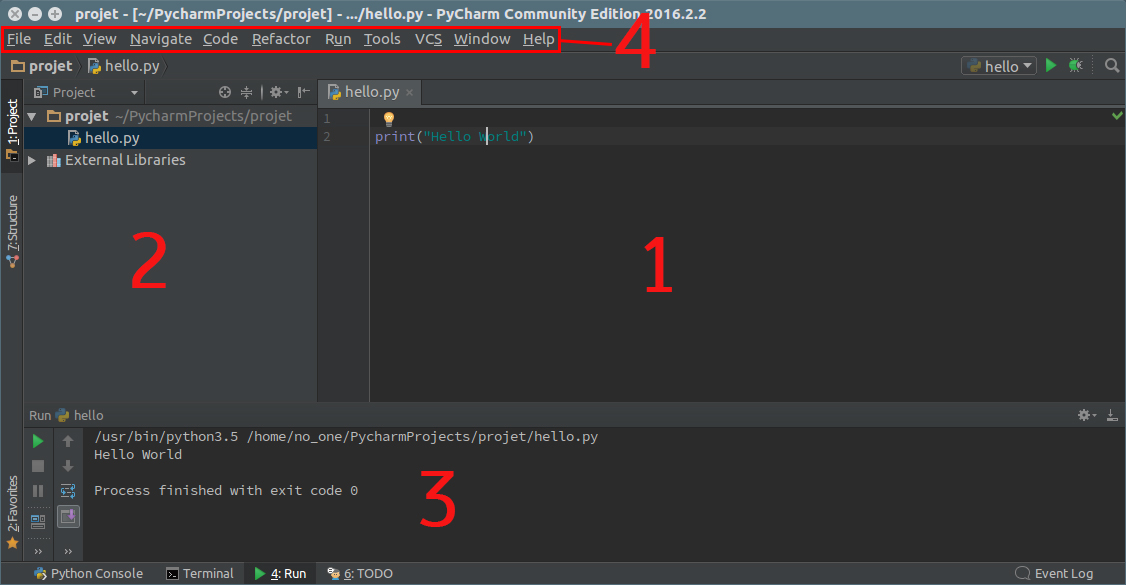
\includegraphics[width=\linewidth]{img/8_pycharm.png}
            \caption{Pycharm}
            \label{pycharm}
        \end{figure}

        PyCharm est composé essentiellement de 4 partie :
        \begin{description}
            \item[La zone principale (1):] c'est dans cette zone où on écrira notre code source (nos instructions).
            \item[La liste des fichiers du projet (2):] dans cette zone on peu voir tous les fichiers de notre projet.
                On voit bien que le projet présenté dans la \autoref{pycharm} contient un seul fichier seulement.
            \item[La zone d'affichage (3):] c'est cette zone qui nous affichera le résultat d'exécution de notre
                programme, où les éventuelles erreurs s'il y en a.
            \item[La barre d'outils (4):] elle contient de nombreux boutons qui font différentes choses : exécuter
            le projet, configurer l'IDE \ldots\ etc, mais nous on utilisera que quelques boutons.
        \end{description}

        \subsubsection{Installer Python et PyCharm sous Ubuntu Linux}
            Python est installé par défaut dans toute les distributions Linux. Par contre, l'IDE PyCharm il
            faut l'installer. Pour cela, il suffit d'ouvrir un terminal (Ctrl+alt+t) et exécuter ces commandes :
            \begin{lstlisting}[language=bash, style=code, numbers=none]
sudo add-apt-repository ppa:ubuntu-desktop/ubuntu-make -y
sudo apt-get update
sudo apt-get install ubuntu-make -y
umake ide pycharm
            \end{lstlisting}

            Il vous demandera après de choisir un emplacement pour l'installation, tapez juste entrer sans rien changer.

            \begin{figure}[H]
                \centering
                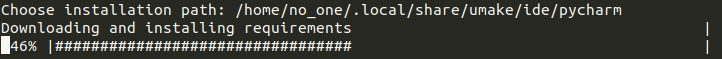
\includegraphics[width=\linewidth]{img/8_1_installer_pycharm.png}
                \caption{Installation PyCharm}
            \end{figure}

            Et voila, PyCharm est installé sur votre machine. Il suffit juste de le lancer en appuyant le bouton
            windows (\autoref{button_windows}) et tapez \code{pycharm} (\autoref{launch_pycharm}) puis tapez entrer.

            \begin{figure}[H]
                \centering
                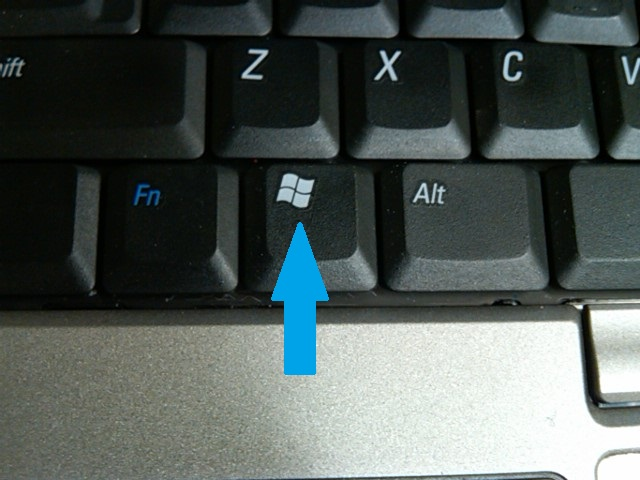
\includegraphics[width=0.5\linewidth]{img/8_windows_button.jpg}
                \caption{Bouton windows}
                \label{button_windows}
            \end{figure}

            \begin{figure}[H]
                \centering
                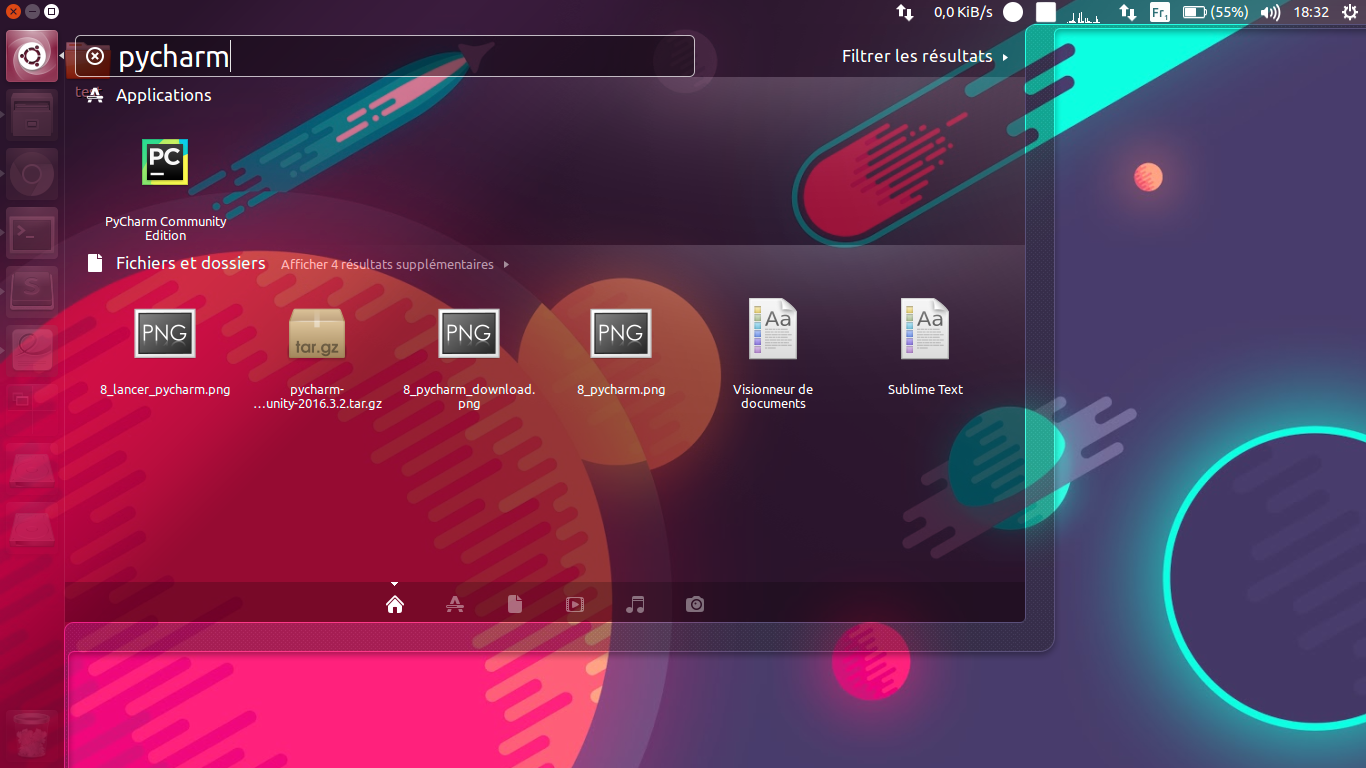
\includegraphics[width=\linewidth]{img/8_lancer_pycharm.png}
                \caption{Lancer PyCharm}
                \label{launch_pycharm}
            \end{figure}
        \subsubsection{Installer Python et PyCharm sous Windows}
            Python n'est pas installé par défaut sur Windows, donc il faut installer Python et l'IDE PyCharm.

            Pour installer Python, visitez ce lien
            \href{https://www.python.org/downloads/}{https://www.python.org/downloads/} et télécharger la
            dernière version de Python (au moment du déroulement de la formation, c'est la version \code{3.6}).
            Installez là quand vous finissez le téléchargement.

            \begin{figure}[H]
                \centering
                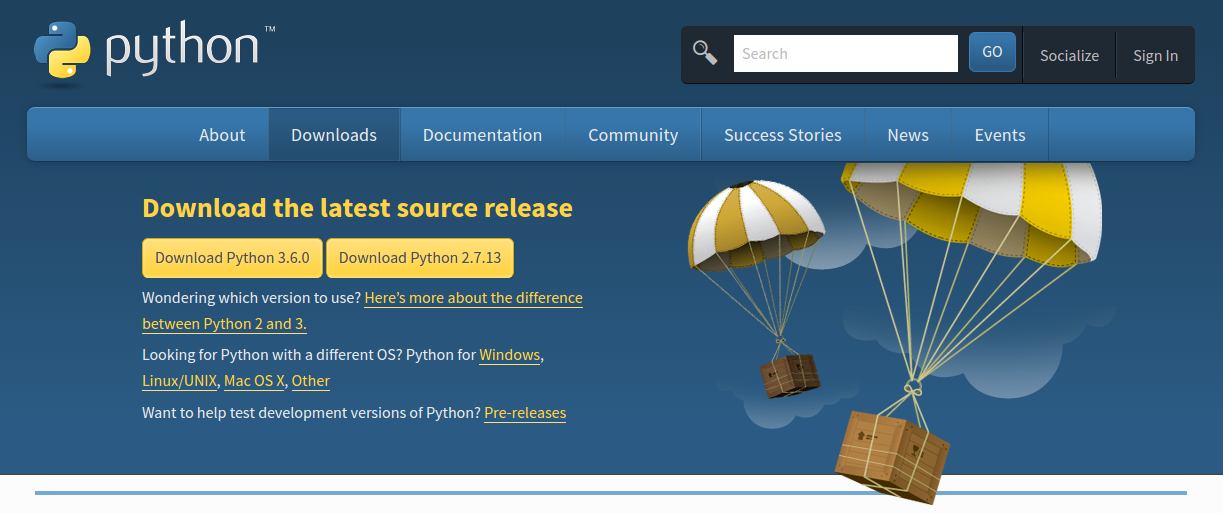
\includegraphics[width=\linewidth]{img/8_python_download.png}
                \caption{Lien de téléchargement de Python}
            \end{figure}

            Pour PyCharm, télécharger la version \code{community} sur ce lien \href{https://www.jetbrains.com/pycharm/download/}{https://www.jetbrains.com/pycharm/download/} (\autoref{site_pycharm}) et installez là.

            \begin{figure}[H]
                \centering
                
\includegraphics[width=\linewidth]{img/8_pycharm_download.png}
                \caption{Lien de de téléchargement PyCharm}
                \label{site_pycharm}
            \end{figure}

\clearpage

    \subsection{Hello World}
        Nous allons écrire maintenant notre premier programme. Un programme petit et simple pour comprendre le
        fonctionnement de ce langage fascinant.

        On commence par créer un nouveau projet en cliquant sur la barre d'outils sur \code{File -> New Project}. Ensuite on choisis où on veut placer notre projet, et la version de l'interpréteur qu'on veut utiliser
        (\autoref{pycharm_new_project}). Choisissez n'importe quelle version 3.x disponible sur votre ordinateur
        (Pour moi, j'utilise la version 3.5).

        \begin{figure}[H]
            \centering
            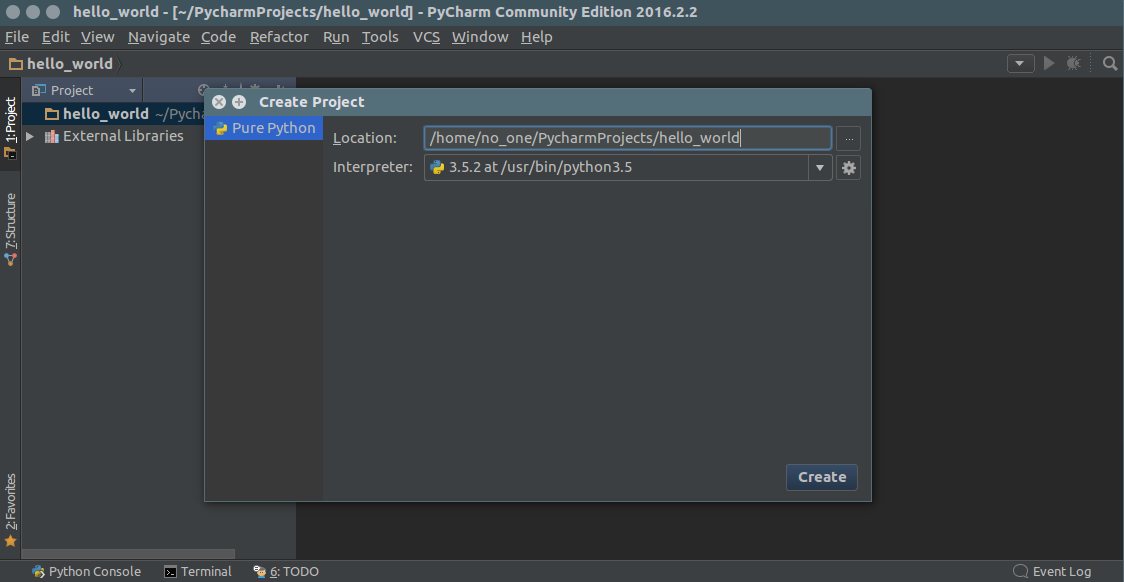
\includegraphics[width=\linewidth]{img/9_new_project.png}
            \caption{Création d'un nouveau projet}
            \label{pycharm_new_project}
        \end{figure}

        On a crée notre projet, mais ce dernier est vide, il ne contient aucun fichier. Nous allons maintenant ajouter
        un fichier où nous allons écrire nos instructions (programmes). On fait un clique sur la barre d'outils sur
        \code{File -> New} et on choisit \code{Python File}. On lui donne un nom à notre fichier, et on clique sur
        \code{OK} (\autoref{new_file}).

        \begin{figure}[H]
            \centering
            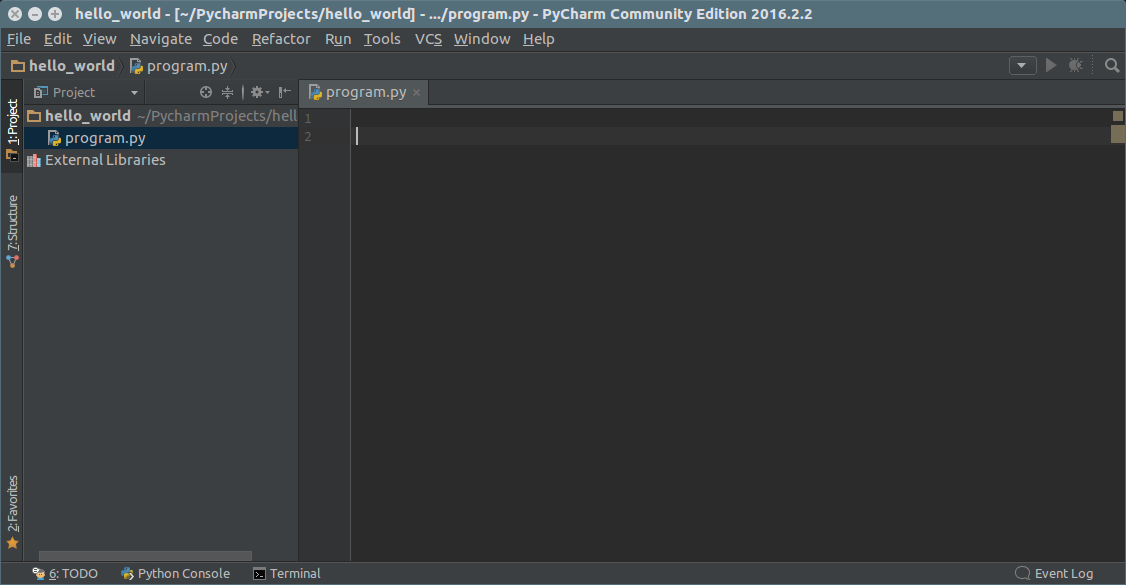
\includegraphics[width=\linewidth]{img/10_new_file.png}
            \caption{Création d'un fichier pour écrire les instructions}
            \label{new_file}
        \end{figure}

        Dorénavant, je vais seulement vous affiché les codes que vous devez écrire dans la zone principale (la zone
        \textbf{1}, \autoref{pycharm}).

        On arrive maintenant à la programmation, voici votre premier programme :
        \begin{lstlisting}[style=code]
print("Hello World!")
        \end{lstlisting}

        Écrivez ce code source dans la zone principale (zone \no1 \autoref{pycharm}), et demandez à PyCharm
        d'exécuter notre programme en cliquant sur la barre d'outils sur \code{Run -> Run}, et on choisit le fichier
        à exécuter (on en a un seul dans notre cas). Voici le résultat de l'exécution :

        \begin{lstlisting}[style=exec_result]
/usr/bin/python3.5 /home/no_one/PycharmProjects/hello_world/program.py
Hello World!

Process finished with exit code 0
        \end{lstlisting}

        Alors, la ligne que nous avons écrit dans l'IDE \code{print("Hello World!")} est une instruction qui demande
        à l'ordinateur d'afficher \code{Hello World!} à l'écran. Nous pouvons écrire n'importe quoi à la place de
        \code{Hello World!} et l'ordinateur se chargera d'afficher le message que nous avons demandé.

        Avant de continuer, nous allons détaillé ce que PyCharm nous a affiché :
        \begin{description}
            \item[/usr/bin/python3.5] c'est le chemin vers l'interpréteur python que PyCharm a utilisé pour
                exécuté notre programme. La majorité des programmes sous \emph{Linux} sont installés dans le dossier
                \code{/usr/bin/}\ .
            \item[/home/no\_one/PycharmProjects/hello\_world/program.py] ça c'est notre fichier (là où on est entrain
                d'écrire notre code source). Donc d'après cette ligne, on comprend que \code{python3.5} est entrain
                d'exécuter ce fichier.
            \item[Hello World!] c'est le message que nous avons demandé à python d'affiché (on voit qu'il a bien
                obéi).
            \item[Process finished with exit code 0] ceci est un message affiché par \code{PyCharm} pour nous indiquer
                que notre programme s'est terminé avec succès.
        \end{description}

        Donc, \code{print()} est l'instruction responsable d'afficher un message à l'écran. On lui donne entre
        les \code{""} le message qu'on veut afficher.
        Essayez de Remplacer \code{Hello World!} par \code{Salut tout le monde} et ré-exécuté pour voir le nouveau résultat.

        \subsubsection{Les commentaires}
            Avant de terminer cette section avec un TP, nous allons parler des commentaires.
            Dans n'importe quel langage de programmation (y compris python), on a la possibilité d'écrire des commentaires.

            Alors c'est quoi les commentaires ? Ce sont des bouts de textes qu'on écrit dans notre code source et qui
            permettrons d'expliquer le fonctionnement de notre code source. Ça peut vous semblez bizarre et inutile, mais
            sachez que c'est très commun qu'on revient à notre programme après quelques semaines pour l'améliorer
            ou pour le modifier, et sans les commentaires on sera obligé de tout repenser du début. Ne vous faites pas
            avoir par le fait que c'est vous qui a crée ce programme, car même si vous comprenez tous sur votre
            programme maintenant, vous oublierai après un certain temps.

            Les commentaires ne serviront pas seulement à comprendre son code seulement, mais c'est très utile aussi
            quand vous travaillez en groupe pour crée un programme. Quand vous utilisez les commentaires, vous ne serrez
            pas obligé d'expliquer la partie que vous avez écrit à vos camarades.

            J'insiste exprès sur le fait d'utiliser les commentaires, ils sont très très utiles et indispensables.

            Alors, on sait ce que sont les commentaires, mais comment les utiliser avec \code{python} ? Voici
            un exemple sans plus tardé :
            \begin{lstlisting}[style=code]
# Cette instruction affiche Hello World! a l'ecran.
print("Hello World!")
            \end{lstlisting}

            Les commentaires commence par un \code{\#}, tous ce qui suit ce caractère est ignoré par \code{python}.
            Donc on peut écrire autant de ligne de commentaire qu'on veut, il faut juste précédé chaque ligne avec un
            \code{\#}.

        \subsubsection{Exercice 1}
            Bon, on a assez bavardé, vous allez écrire votre vrai premier programme crée par vous même.
            Voici l'exercice :
            \begin{itemize}
                \item Créez un nouveau projet et nommé le ``exercice 1''.
                \item Créez un fichier dans ce projet où nous allons mettre notre code source. nommé ce fichier
                    ``main''.
                \item Débrouillez vous pour que le programme affiche :
                    \begin{lstlisting}[style=exec_result, breaklines=false]
Salut tout le monde.
On est dans une formation python, et on va cree des programmes super cool :D.
                    \end{lstlisting}
                \item N'oubliez pas d'utiliser les commentaires pour expliquer votre code.
            \end{itemize}

        \subsubsection{Solution de l'exercice}
            \begin{lstlisting}[style=code, breaklines=false]
# Ces deux instructions affiche des messages a l'ecran.
print("Salut tout le monde.")
print("On est dans une formation python, et on va cree des programmes super cool :D.")
            \end{lstlisting}

\clearpage

    \subsection{Les variables}
        Les variables sont une notion fondamentale en informatique et il sont utilisé dans tous les langages
        de programmation sans exception. Il ont plusieurs définitions, mais je pense que celle qu'on va voir est la plus simple.

        En faite, votre ordinateur est une armoire géante qui contient des millions et des millions de tiroirs, et
        chaque tiroir
        est utilisé pour stocker des informations. Donc quand vous voulez stocké une information (disons votre age)
        pour l'utilisé plus tard dans votre programme, vous demandez à votre ordinateur de vous allouer un tiroir.
        Ce tiroir vous serra allouer jusqu'à la fin de votre programme.

        \begin{figure}[H]
            \centering
            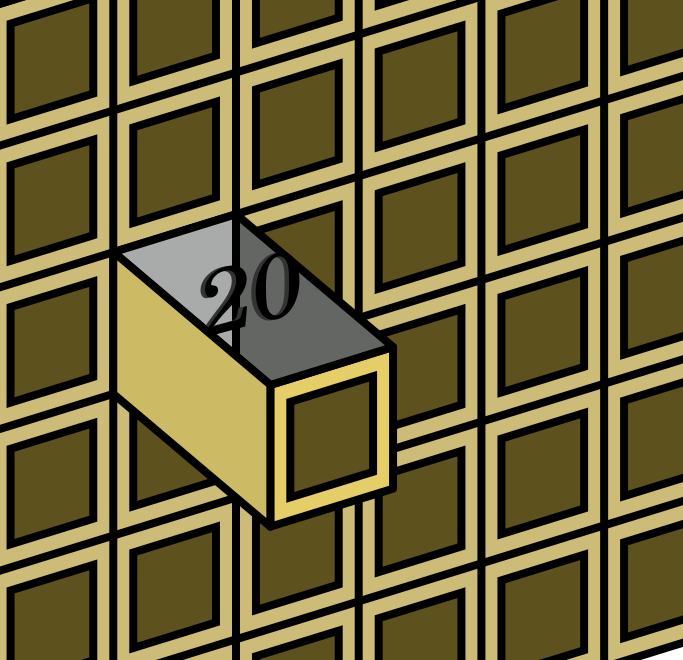
\includegraphics[width=0.5\linewidth]{img/13_variable.png}
            \caption{Une tiroir qui stocke notre information}
        \end{figure}

        Ce tiroir est le votre, vous pouvez placez des information dedans, les consulter, les retirer.

        \questionbox{Donc, où sont les variables dans tous ça ??}

        Les variables sont des noms qu'on associé aux tiroirs que nous
        avons demandé. Donc, dans l'exemple précédent, nous avons utilisé un tiroir pour stocker un age, donc nous
        allons nommé ce tiroir \code{age}. Et à chaque fois qu'on veut consulter ou modifier le contenu de ce tiroir,
        (supposons vous avez oublié votre age) on utilise le mot \code{age}.

        \begin{figure}[H]
            \centering
            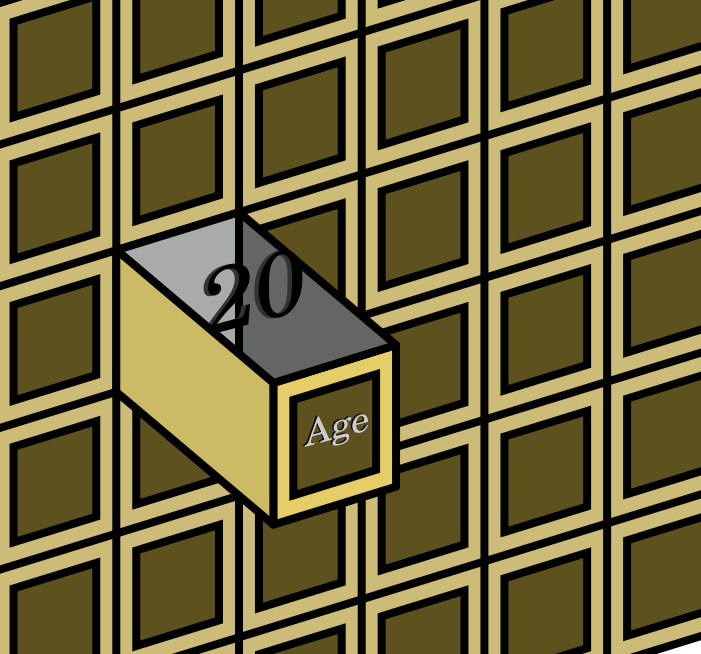
\includegraphics[width=0.5\linewidth]{img/14_variable.png}
            \caption{Une tiroir qui stocke notre information, et qui est accessible par le nom age}
        \end{figure}

        \subsubsection{Créer et utiliser les variables avec python}
            Pour créer une variable avec python, rien de plus simple. Il suffit d'écrire le nom de notre variable :
            \begin{lstlisting}[style=code]
age = 20
            \end{lstlisting}

            Avec cette instruction, nous avons maintenant un tiroir réservé à nous, ce tiroir est accessible en
            écrivant le mot \code{age} dans python.

            Si on veut voir le contenu de notre tiroir (variable), on peut utiliser
            l'instruction qu'on a vu précédemment \code{print()} (celle qui permet d'afficher à l'écran) :
            \begin{lstlisting}[style=code]
age = 20
# Cette instruction va afficher mon age.
print(age)
            \end{lstlisting}

            On peut même modifier le contenu de notre variable à n'importe quel moment :
            \begin{lstlisting}[style=code]
age = 20
# Cette instruction va afficher mon age.
print(age)

# Ces deux instructions vont me rendre plus vieux,
# et afficher mon nouveau age.
age = 30
print(age)
            \end{lstlisting}

            Voici ce qui nous serra affiché par PyCharm après l'exécution de notre programme :

            \begin{figure}[H]
                \centering
                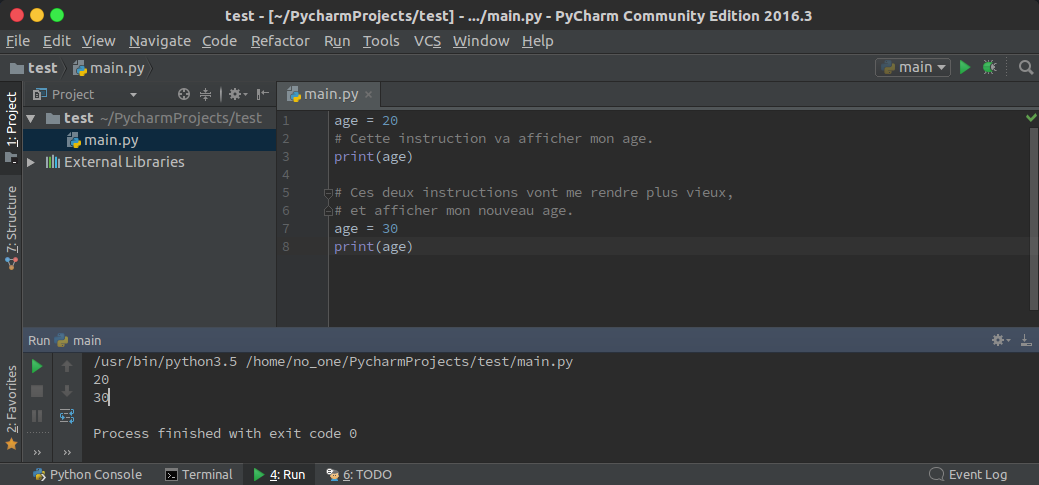
\includegraphics[width=\linewidth]{img/15_affiche_variables.png}
                \caption{Affichage de la variable age}
            \end{figure}

        \subsubsection{Quel genre d'information on peut stocker dans nos variables}
            Il existe essentiellement 3 types d'information qu'on peut stocker dans les variables :
            \begin{description}
                \item[Les entiers :] comme ce que nous avons stocké dans la variable \code{age} que nous avons
                    utilisé jusque là. Les entiers sont appelé \code{int} en python.
                \item[Les valeurs décimales :] des nombres à virgules, (comme : 3.453). Ces nombres sont appelé
                    \code{float} en python. Exemple :
                    \begin{lstlisting}[style=code]
pi = 3.14
                    \end{lstlisting}
                \item[Du texte :] on les appels les chaînes de caractères ou \code{str} en python. On les définit on les
                    entourant par \code{""} ou \code{''}. Exemple :
                    \begin{lstlisting}[style=code]
prenom = "Amine"
prenom2 = "Moustapha"
nom = 'Malaoui'
                    \end{lstlisting}
            \end{description}

        \subsubsection{Afficher les variables}
            Vous savez déjà qu'on peut afficher le contenu d'une variable avec \code{print()}, mais ce que vous
            ne savez pas c'est que \code{print()} permet d'afficher plusieurs variables à la fois. Il suffit
            juste de les séparer par des \code{,} :
            \begin{lstlisting}[style=code]
# Je cree mes variables
prenom = "Amine"
nom = "Malaoui"

print("Salut, je m'appelle", prenom, nom)
            \end{lstlisting}

            En exécutant notre programme, PyCharm nous affichera ça :

            \begin{lstlisting}[style=exec_result]
/usr/bin/python3.5 /home/no_one/PycharmProjects/test/main.py
Salut, je m'appelle Amine Malaoui

Process finished with exit code 0
            \end{lstlisting}

        \subsubsection{Récupérer une saisie}
            Ce que nous avons fait jusque là c'est de crée nos variables, et de les données des valeurs directement dans
            le code source. Ce que nous allons apprendre maintenant c'est de demander de l'utilisateur
            de donner une valeur à notre variable au cours d'exécution.

            Pour cela on va utiliser l'instruction de récupération de saisie, qui est \code{input()} :
            \begin{lstlisting}[style=code]
# On demande a l'utilisateur de nous donner son prenom,
# et on stock son prenom apres dans la variable prenom.
prenom = input("Veuillez entrer votre prenom : ")

# On dit bonjour a l'utilisateur.
print("Bonjour", prenom)
            \end{lstlisting}

            Ce que fait ce code c'est qu'il affiche à l'utilisateur \code{Veillez entrer votre prenom :}, et il lui
            donne la main après pour qu'il entre son prénom. Son prénom est maintenant stocker dans la variable
            \code{prenom}. Voila ce que PyCharm nous affiche après l'exécution :
            \begin{figure}[H]
                \centering
                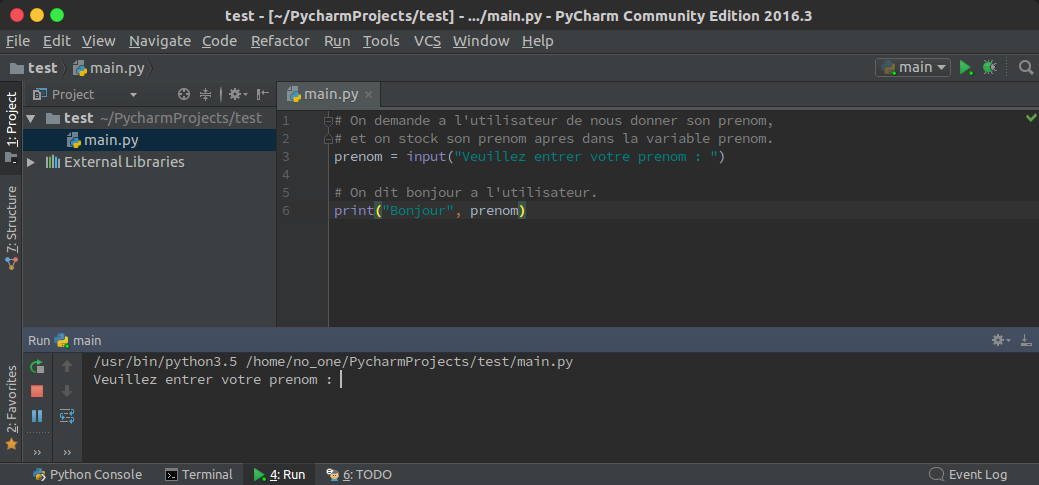
\includegraphics[width=\linewidth]{img/16_input.png}
                \caption{PyCharm attend qu'on entre le prénom}
            \end{figure}

            Dès que l'utilisateur entre son nom et tape \code{Entrée}, PyCharm lui affiche \code{Bonjour} suivi
            du prénom de l'utilisateur :
            \begin{figure}[H]
                \centering
                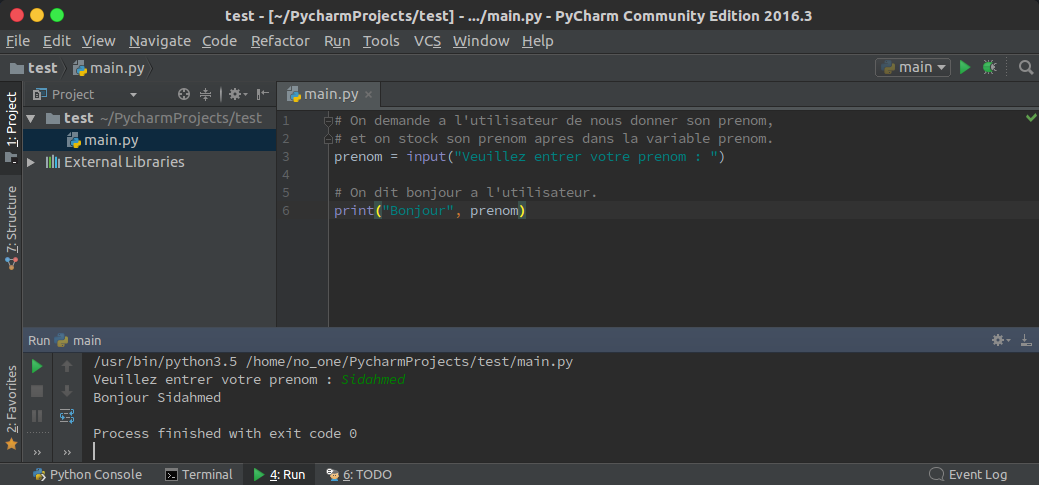
\includegraphics[width=\linewidth]{img/17_input.png}
                \caption{PyCharm affiche Bonjour suivi du prénom}
            \end{figure}

        \subsubsection{Comment nommé les variables}
            On va parler de la meilleur manière de nommé les variables avant de finir cette partie.
            vous avez juste quelques règles à suivre, et tout passera à merveille :
            \begin{itemize}
                \item Le nom d'une variable doit commencer par une lettre. Exemple :
                    \begin{lstlisting}[style=code]
# Faux
1prenom = 20

# Juste
prenom1 = 20

# Juste
prenom = 20
                    \end{lstlisting}

                \item Donner toujours des noms explicites à vos variables. C'est à dire en observant le nom de votre
                    variable, il faut que vous serrez capable de comprendre son fonctionnement. Croyez moi, ça vous
                    sera extrêmement utiles quand vous réexaminer votre code. \\Par exemple, si on veut stocker
                    l'age d'un utilisateur :
                    \begin{lstlisting}[style=code]
# Faux, car c'est pas claire que x designe un age.
x = 20

# Juste
age = 20
                    \end{lstlisting}

                \item Si le nom de votre variable doit être composé de plusieurs mots, séparer les mots par un \code{\_}.
                    Exemple :
                    \begin{lstlisting}[style=code]
# Faux
notedemath = 15

# Juste
note_de_math = 15
                    \end{lstlisting}

                \item Et enfin, n'utilisez pas de caractères avec accents (comme \code{é}, \code{è}, \code{à} \ldots)
                    car ça peut vous posez des problèmes plus tard.
            \end{itemize}

            Enfin, nous avons terminé de parler sur les variables. Nous allons faire un petit exercices avant de passer
            à la section suivante.
        \subsubsection{Exercice 2}
            Ne sautez pas ces exercices, c'est très important de pratiquer en informatique.

            Voici l'énoncé de l'exercice :
            \begin{itemize}
                \item Créez un nouveau projet et nommé le ``exercice 2'', et créez un fichier ``main.py'' dans ce
                    projet.
                \item Débrouillez vous pour que le programme demande le ``prenom'', ``nom'' et ``age'' de l'utilisateur.
                    Puis affichez tous ça dans une phrase du genre : \code{Tu t'appelles Yanis Khelloufi et tu as 22 ans.}.
            \end{itemize}


\clearpage

    \subsection{les opérateurs arithmétique}
        Les ordinateurs sont des vrai machines à calcul, c'est ce qu'il savent faire le mieux. Donc dans cette partie
        nous allons apprendre à faire des calcules avec python.

        Il y a dans python 5 symboles qui nous permettent de faire des opérations arithmétique :
        \begin{itemize}
            \item \code{+} fait l'addition.
            \item \code{-} fait la soustraction.
            \item \code{*} fait la multiplication.
            \item \code{/} fait la division entière.
            \item \code{//} fait la division euclidienne.
            \item \code{\%} donne le reste de la division euclidienne (on appel ça le \emph{modulo}).
            \item \code{**} calcul la puissance.
        \end{itemize}

        \subsubsection{Addition, soustraction, multiplication}
            Pour l'addition et la soustraction et la multiplication, rien de plus simple, on utilise seulement
            les symboles approprié, et tout passe à merveille. Exemple :
            \begin{lstlisting}[style=code]
x = 10 + 5
y = 21 - 7
z = 9 * 9

# Ceci affichera : 15 14 81
print(x, y, z)
            \end{lstlisting}

        \subsubsection{Division entière et Division euclidienne}
            Pour voir la différence, un exemple vaut mieux qu'un long discours :
            \begin{lstlisting}[style=code]
division_entiere = 10 / 3
division_euclidienne = 10 // 3

# Ceci affichera : 3.3333333333333335  3
print(division_entiere, division_euclidienne)
            \end{lstlisting}

        \subsubsection{Modulo (reste de la division euclidienne)}
            Exemple :
            \begin{lstlisting}[style=code, breaklines=false]
x = 10 % 3

# Ceci nous affichera 1. Car le reste de la division de 10 par 3 donne 1.
print(x)
            \end{lstlisting}
        \subsubsection{La puissance}
            Rien de plus simple. Exemple :
            \begin{lstlisting}[style=code]
x = 5 ** 2

# Ceci affichera 125
print(x)
            \end{lstlisting}


        \subsubsection{Opérations entre variables}
            Sachez bien que toutes les opérations que nous avons vu précédemment sont aussi applicables sur les variables.
            Donc on peut faire des calculs entres variables. Exemple :
            \begin{lstlisting}[style=code]
a = 10
b = 15
resultat = a + b

# Ceci affichera : 10 + 15 = 25
print(a, "+", b, "=", resultat)
            \end{lstlisting}

        \subsubsection{Bonus}
            Dans la majorité des autres langages de programmation, pour permuter deux variables
            (échanger leurs contenus), il faut toute une série d'opérations.

            Exemple : disons on a les variables \code{a} et
            \code{b}, pour permuter leurs valeurs dans les autres langages de programmation, il faut faire ça :
            \begin{lstlisting}[style=code]
# Il faut ces trois opérations pour permuter les valeurs
# de a et b
variable_temporaire = a
a = b
b = variable_temporaire
            \end{lstlisting}

            Alors en python, il suffit juste de faire :
            \begin{lstlisting}[style=code]
# cette instruction permutent les valeurs de a et b
a, b = b, a
            \end{lstlisting}

            Vous pouvez créer les variables \code{a} et \code{b}, essayez ce code, et afficher ces deux variables
            pour voir le résultat.
        \subsubsection{Un petit problème !}
            Essayez ce code :
            \begin{lstlisting}[style=code, breaklines=false]

date_de_naissance = input("Veuillez entrer votre date de naissance : ")
age = 2017 - date_de_naissance

print("Votre avez", age, "ans")
            \end{lstlisting}

            Malheureusement, PyCharm n'a pas pu exécuter notre programme, et il nous affiche une erreur :
            \begin{lstlisting}[style=exec_result]
/usr/bin/python3.5 /home/no_one/PycharmProjects/test/main.py
Veuillez entrer votre date de naissance : 1994
Traceback (most recent call last):
  File "/home/no_one/PycharmProjects/test/main.py", line 3, in <module>
    age = 2017 - date_de_naissance
TypeError: unsupported operand type(s) for -: 'int' and 'str'

Process finished with exit code 1
            \end{lstlisting}

            Ce qui s'est passé c'est que l'instruction \code{input()} récupère la saisie sous forme de texte. Donc
            ce qu'elle a stocké dans la variable \code{date\_de\_naissance} n'est pas le nombre \code{1994} mais plutôt
            le texte (chaînes de caractères) \code{"1994"}. Donc quand Python arrive à l'instruction de la soustraction,
            il essaye de soustraire un texte d'un entier, et là ça plante, car ce n'est pas possible.

            La solution consiste à convertir notre variable \code{date\_de\_naissance} en un entier. C'est extrêmement
            simple, il suffit juste d'utiliser l'instruction \code{int()}. Voici à quoi rassemblerai notre nouveau
            code source :
            \begin{lstlisting}[style=code, breaklines=false]
date_de_naissance = input("Veuillez entrer votre date de naissance : ")
# On converti notre variable en un entier.
date_de_naissance = int(date_de_naissance)

age = 2017 - date_de_naissance

print(age)
            \end{lstlisting}

            Et cette fois, le programme marche à merveille.

            N'oubliez pas, dorénavant, quand vous utilisez \code{input()},
            mettez en tête qu'elle récupère la saisie sous forme de texte. Pensez donc à convertir votre variable si
            vous voulez l'utiliser comme entier (utilisez \code{int()}) ou nombre à virgule (utilisez \code{float()}).

        \subsubsection{Exercice 3}
            Voici l'énoncé de l'exercice :
            \begin{itemize}
                \item Créez un nouveau projet et nommé le ``exercice 3'', et créez un fichier ``main.py'' dans ce
                    projet.
                \item Demandez l'age de l'utilisateur, et dite lui à quel année il aura 100 ans.
            \end{itemize}

\clearpage

    \subsection{Les conditions}
        Les conditions sont des concepts fondamentaux de n'importe quel langage de programmation. Mais il sont un petit
        peu difficile à comprendre au début, mais vous verrez que dés que vous comprenez les conditions, vous serrai
        déjà capable de crée un programme disons intelligent et qui réagit selon la situation.

        Par exemple : vous pouvez demander l'age de l'utilisateur, et puis lui affiche un message selon son age. Si il a
        plus de 18 ans, vous lui affichez \code{Vous êtes majeur}, sinon vous lui affichez \code{Vous êtes mineur}.

        Avant de commencer de parler des conditions, il y a un ensemble de symbole que vous devez apprendre par cœur.
        Ces symboles sont utilisés pour réaliser les conditions :

        \begin{table}[h] % Le 'h' pour que la tableau soit dans la position qu'on vient d'indiquer.

            \centering
            \begin{tabular}{|c|l|}
            \hline
            \textbf{Symbole} & \textbf{Signification} \\
            \hline
            == & est égal à \\
            \hline
            > & est supérieur à \\
            \hline
            < & est inférieur à \\
            \hline
            >= & est supérieur ou égal à \\
            \hline
            <= & est inférieur ou égal à \\
            \hline
            != & est différent de \\
            \hline
            \end{tabular}

            \caption{Symboles de comparaison} % On donne une légende à notre tableau
        \end{table}
        % Bon, jusque là, votre programme faisait toujours la même chose. Par exemple, il demande l'age de l'utilisateur, et
        % il le lui affiche, et quand vous le relancez à nouveau, il refait la même chose.

        % Avec les conditions, vos
        % programmes feront des choses différentes selon le contexte. Par exemple si l'utilisateur a plus de 18 ans, on
        % lui affiche \code{T'es majeur}, sinon on lui affiche \code{T'es mineur}.

        \subsubsection{Le if}
            Pour réaliser une condition minimal en python, il faut juste suivre un schéma simple, le voici :
            \begin{lstlisting}[style=code]
if condition :
    instruction1
    instruction2
    .
    .
    .
    instructionN
            \end{lstlisting}

            Donc, la condition \code{condition} sera évalué par python, si elle est vrai, il exécute toutes les instruction
            qui se trouvent dans le bloc du \code{if}, et si elle est fausse, alors il va sauter toutes les instructions
            qui se trouvent dans le bloc du \code{if}.

            \importantbox{
            Attention, il faut que les instructions soient décalé par rapport
            à notre \code{if} comme  le montre l'exemple précédent. C'est comme ça que python comprend quelles sont les
            instruction qui appartiennent au \code{if} et quelles sont les instructions qui appartient au programme principale.
            }

            \notebox{Juste pour titre informatif, ce décalage est appelé \emph{Indentation}, et l'ensemble d'instruction qui se
            trouvent dans le \code{if} est appelé \emph{Un bloc de code}.}

            On donne un exemple :
            \begin{lstlisting}[style=code, breaklines=false]
age = 20

# On test si l'age est superieur a 18 pour afficher un message.
if age > 18 :
    print("Vous etes majeur")

print("Au revoir")
            \end{lstlisting}

            Si on exécute ce code, on voit que le message \code{Vous etes majeur} est affiché, et même le message
            \code{Au revoir} est affiché. Mais si on modifie l'age pour lui donner une valeur inférieur à \code{18}, alors
            seulement le message \code{Au revoir} est affiché, car cette instruction n'est pas inclut dans le bloc du \code{if}.

        \subsubsection{Le else}
            Pour enrichir encore plus notre code, on peut utilisé le \code{else}. Ça permet de désigner un bloc sinon, ce
            bloc sera exécuté si la condition évalué dans le \code{if} est fausse. Un exemple :
            \begin{lstlisting}[style=code, breaklines=false]
age = 20

# Si l'age est supérieur a 18 on affiche : Vous êtes majeur.
# Sinon (c'est a dire l'age inférieur ou égale a 18) alors
# on affiche : Vous êtes mineur.
if age > 18 :
    print("Vous êtes majeur")
else :
    print("Vous êtes mineur")

print("Au revoir")
            \end{lstlisting}

            Si on modifie l'age pour qu'il soit inférieur ou égale à \code{18}, on remarquera que cette fois c'est le message
            \code{Vous etes mineur} qui sera affiché. Le message \code{Au revoir} est toujours affiché, car il n'appartient
            ni au \code{if} ni au \code{else}.

        \subsubsection{Le elif}
            Le \code{elif} est une abréviation de \code{else if} qui veut dire \emph{Sinon Si}. Il se situe entre le
            \code{if} et le \code{else}, et ça permet de tester une autre condition.

            Ça peut vous semblez abstrait, mais un exemple va éclaircir le concept :
            \begin{lstlisting}[style=code, breaklines=false]
age = 20

# Si l'age est superieur a 70 alors on affiche : Salut papi
# Sinon si l'age est superieur a 40 alors on affiche : Salut monsieur
# Sinon si l'age est superieur a 18 alors on affiche : Salut jeune
# Sinon on affiche le message qui se trouve dans le else.
if age > 70 :
    print("Salut papi")
elif age > 40 :
    print("Salut monsieur")
elif age > 18 :
    print("Salut jeune")
else :
    print("Tu n'appartient à aucune catégorie, dégage -_-")

# Ce message est toujours affiché.
print("Au revoir")

            \end{lstlisting}

            En utilisant le \code{elif}, on pourra re-tester la valeur de la variable age une autre fois. Amusez vous
            à changer la valeur de la variable \code{age}, et vous verrez qu'à chaque fois l'un des 4 messages est affiché.

            \importantbox{
            Faites très attention, un seule bloc d'instruction est exécuté parmi tous ces 4 blocs. Donc si on donne
            la valeur \code{70} à notre variable \code{age}, seul bloc de code du \code{if} sera exécuté, et tout les
            autres \code{elif} et le \code{else} seront ignoré.}

        \subsubsection{Comparez les chaînes de caractères}
            Sachez que c'est testes qu'on vient de voir ne sont pas applicables seulement au nombres, on peut aussi
            les appliquer au chaînes de caractères. Exemples :

            \begin{lstlisting}[style=code, breaklines=false]
mot_de_passe = input("Veuillez entrer votre mot de passe: ")

if mot_de_passe == "MonSuperMotDePasse" :
    print("Bienvenu")
else
    print("Dégaaaaaaaaaage imposteur")
            \end{lstlisting}
        \subsubsection{Plusieurs conditions à la fois}
            Jusque là, nous avons tester une seule condition dans le \code{if} ou le \code{elif}, par exemple "Si
            l'age est supérieur à 18". Mais comment faire si on veut tester "Si l'age est supérieur à 18 et
            inférieur à 40 au même temps" ??
            Pour cela, il suffit d'utiliser les opérateurs logique. Ces opérateurs permettent de combiner plusieurs
            condition à la fois.

            Il y a un ensemble de règles à apprendre pour réaliser cela :
            \begin{table}[H]
                \centering
                \begin{tabular}{|c|c|}
                    \hline
                    \textbf{Symbole} & \textbf{Signification} \\
                    \hline
                    and & ET \\
                    \hline
                    or & OU \\
                    \hline
                    not & NON \\
                    \hline
                \end{tabular}
                \caption{Les opérateurs logiques}
            \end{table}

            Voici quelques exemples du fonctionnement de ces opérateurs :
            \begin{lstlisting}[style=code]
# Si l'age est supérieur à 18 et inférieur à 40 au même temps.
if age >= 18 and age <= 40:
    # Les instructions
            \end{lstlisting}

            \begin{lstlisting}[style=code, breaklines=false]
# Si on est Samedi ou Vendredi alors on entre dans le bloc du if.
if jour == "Samedi" or jour == "Vendredi" :
    # Pas d'études
            \end{lstlisting}

            \begin{lstlisting}[style=code]
# Le 'not' est utilisé pour exprimé la négation d'une condition.
# Ça se traduit en : si l'age n'est pas supérieur à 18.
if not age > 18 :
    # Les instructions
            \end{lstlisting}

            Sachez qu'on peut combinez les opérateurs logiques entres eux, mais pour cela vaut mieux
            utiliser les parenthèses pour exprimer la priorité. Exemple :
            \begin{lstlisting}[style=code]
if (jour == "Samedi" or jour == "Vendredi") and chaleur < 35 :
    # Sortir de la maison
            \end{lstlisting}

        \subsubsection{Les booléens}
            Il y a un autre type de variables dont je ne vous ai pas parlé avant pour ne pas vous en charger.
            Ce type de variable est appelé \emph{Booléen} (\code{bool} en python) et il est très
            utilisé dans les conditions et les boucles.

            Les booléens sont des variables qui peuvent contenir une de deux valeurs seulement : \code{True}
            (qui veut dire vrai) ou \code{False} (qui veut dire faux), et on peut testé directement si ces
            variables sont à vrai dans les conditions :
            % ces variables dans les conditions
            % sans utilisé les opérateurs de comparaisons. Exemple :
            \begin{lstlisting}[style=code]
heureux = True

# Si la variable heureux est vrai, alors on entre dans le if,
# Sinon on entre dans le else.
if heureux :
    print("Je suis heureux aujourd'hui :D")
else :
    print("Que personne ne croise mon regard")
            \end{lstlisting}

            \notebox{Les opérateurs logiques sont applicable sur les booléens. Exemple :}
            \begin{lstlisting}[style=code]
# Ça se traduit en : Si la personne et heureuse et
# le jour et beau alors Sorte de la maison.
if heureux and beau_jour :
    # Sortir de la maison
            \end{lstlisting}

        \subsubsection{Exercice 4}
            Voici l'énoncé de l'exercice :
            \begin{itemize}
                \item Créer un projet nommé le `exercice 4' et créer un fichier `main.py' dedans.
                \item Demandez un nombre de l'utilisateur, et dites lui si ce nombre est paire ou impaire.
            \end{itemize}

\clearpage

    \subsection{Les boucles}
        Si vous avez compris les conditions, les boucles seront un jeu d'enfant. En gros, les boucles servent à répéter
        certaines instructions plusieurs fois, et on a deux boucles dans le langage python :
        \begin{itemize}
            \item La boucle \code{while} qui signifie \emph{tant que}.
            \item La boucle \code{for} qui signifie \emph{pour}.
        \end{itemize}


        \subsubsection{La boucle while}
            % \questionbox{Comment les boucles while sont elles réalisé en python ??}

            La boucle \code{while} permet de répéter un bloc d'instructions \emph{tant que} une condition est vrai.
            Exemple :
            \begin{lstlisting}[style=code]
touche = ""

while touche != "q" :
    touche = input("Tapez q pour sortir : ")

print("Au revoir")
            \end{lstlisting}

            Dans cet exemple, on demande à l'utilisateur d'entrer la lettre \code{q}. Si il reste sage et il fait
            ce que nous le avons demandé, alors on lui laisse sortir de la boucle, sinon on lui redemande à nouveau
            jusqu'à ce qu'il entre la touche \code{q}.

            \notebox{On peut utilisé les booléens avec la boucle \code{while}. Exemple : }
            \begin{lstlisting}[style=code]
heureux = True

while heureux :
    # Continuez de sourire.
            \end{lstlisting}

            On donne un autre exemple de l'utilisation de la boucle \code{while}. Imaginez que votre prof vous
            demande d'écrire un programme qui affiche le message "Ceci est un message très utile" 10 fois,
            vous pouvez faire ça :
            \begin{lstlisting}[style=code]
print("Ceci est un message très utile")
print("Ceci est un message très utile")
print("Ceci est un message très utile")
print("Ceci est un message très utile")
print("Ceci est un message très utile")
print("Ceci est un message très utile")
print("Ceci est un message très utile")
print("Ceci est un message très utile")
print("Ceci est un message très utile")
print("Ceci est un message très utile")
            \end{lstlisting}

            C'est vrai que ça accomplira ce que votre prof a demandé, mais ce n'est ni propre ni pratique. Et imaginez
            encore si cette fois elle vous demande d'afficher ce message 100 fois, ou 1000 fois \ldots on voit bien que
            cette technique n'est plus efficace.

            Ce qu'on peut faire pour réaliser ce que le prof a demandé c'est d'utiliser la boucle \code{while} et un
            \emph{compteur} :
            \begin{lstlisting}[style=code]
# On initialise notre variable qui nous servira de compteur.
i = 0

# Tant que la variable compteur est inférieur à 10 on
# affiche un autre message.
while i < 10:
    print("Ceci est un message très utile")
    # On incrémente notre compteur pour savoir quand s'arrêter.
    i = i + 1
            \end{lstlisting}

            Voici le résultat d'exécution :
            \begin{lstlisting}[style=exec_result]
Ceci est un message très utile
Ceci est un message très utile
Ceci est un message très utile
Ceci est un message très utile
Ceci est un message très utile
Ceci est un message très utile
Ceci est un message très utile
Ceci est un message très utile
Ceci est un message très utile
Ceci est un message très utile
            \end{lstlisting}

            \notebox{La variable \code{i} est souvent utilisé en informatique comme un compteur ou pour parcourir les tableaux
            (on verra ça plus tard). }

            \notebox{En informatique, dans la majorité des cas, on commence nos compteur de \code{0} et pas de \code{1}.
            Ça a une relation avec le parcours des tableaux qu'on verra dans les prochaines sections. Donc si vous voulez
            utilisé un compteur, il faut de préférence commencer de \code{0}.}


        \subsubsection{La boucle for}
            La boucle \code{for} est utilisé uniquement avec les compteurs. C'est une forme compacté de la boucle \code{while}
            précédente. Si on refait l'exemple précédent en utilisant la boucle \code{for} ça nous donne ça :
            \begin{lstlisting}[style=code]
# Ça se traduit en : pour i allant de 0 à 10 (exclus).
for i in range(0, 10):
    print("Ceci est un message très utile")
            \end{lstlisting}

            Dans cet exemple, \code{i} prend chacune des valeurs \code{0}, \code{1}, \code{2}, \code{3}, \code{4}, \code{5},
            \code{6}, \code{7}, \code{8}, \code{9}. Et à chaque fois on affiche le message \code{Ceci est un
            message très utile}.

            Pour voir que \code{i} prend vraiment toute ces valeurs là, on peut afficher la variable \code{i} à chaque
            itération de la boucle :
            \begin{lstlisting}[style=code]
for i in range(0, 10) :
    print(i)
            \end{lstlisting}

            Ce qui nous donne ça :
            \begin{lstlisting}[style=exec_result]
0
1
2
3
4
5
6
7
8
9
            \end{lstlisting}

            On a vu la boucle \code{for}. Maintenant détaillons un peu comment l'utiliser :
            \begin{lstlisting}[style=code]
for i in range(depart, arrivee) :
    print(i)
            \end{lstlisting}

            La variable \code{i} parcourra toute les valeurs en démarrant de la valeur \code{depart} (inclus)
            jusqu'à la valeur \code{arrivee} (exclus). Amusez vous à changer la valeur de \code{depart}
            et \code{arrivee} pour voir quelles sont les valeurs pris par \code{i}.

        \subsubsection{Un bonus de l'utilisation de la boucle for}

            Dans certaines situations, on utilise la boucle \code{for} de cette manière :
            \begin{lstlisting}[style=code]
for i in range(depart, arrivee, pas) :
    print(i)
            \end{lstlisting}

            C'est comme l'utilisation précédente, mais là on a ajouté le \code{pas}. Ce \code{pas} est utilisé pour dire à
            la variable \code{i} combien elle doit sauter à chaque itération de la boucle. Essayez cette exemple et vous
            verrez :
            \begin{lstlisting}[style=code]
for i in range(0, 10, 2) :
    print(i)
            \end{lstlisting}

            L'exécution nous donne ça :
            \begin{lstlisting}[style=exec_result]
0
2
4
6
8
            \end{lstlisting}

            \code{i} démarre de \code{0}, mais à chaque itération de la boucle, elle fait un saut de \code{2}.

        \subsubsection{Exercice 5}
            Voici l'énoncé :
            \begin{itemize}
                \item Créez un projet nommé `exercice 5' et créez un fichier dedans nommé `main.py'.
                \item Demandez à l'utilisateur d'entrer un nombre, et affichez lui tous les diviseurs de ce nombre.
                    Exemple : Si l'utilisateur entre \code{10}, vous lui affichez \code{1}, \code{2}, \code{5}, \code{10}.
            \end{itemize}

\clearpage

    \subsection{Découper le programme en fonctions}
        Jusque là, nous avons écrit toutes nos instructions directement , l'une après l'autre. Maintenant, nous allons
        apprendre à découper nos programmes en petit bouts, et cela grâce aux fonctions.

        \subsubsection{C'est quoi une fonction ?}
            Une fonction est un ensemble d'instructions qu'on groupe ensemble. Cet ensemble d'instructions exécute
            des actions et renvoient un résultat.

            Il vaut mieux que vous comprenez les fonctions avec les exemples, alors on va donner plusieurs exemples
            et on va les expliquer un à un.

        \subsubsection{Fonction simple}

            Voici l'exemple d'une fonction qui calcule le triple d'un nombre :
            \begin{lstlisting}[style=code]
def triple(nombre) :
    resultat = nombre * 3
    return resultat
            \end{lstlisting}

            Et voici comment on va utiliser cette fonction dans notre programme :
            \begin{lstlisting}[style=code]
# Instructions ici
x = triple(7)

# Ceci nous affichera 21
print(x)
            \end{lstlisting}

            Des explications s'impose ici :
            \begin{itemize}
                \item \code{def triple(nombre) :} : \code{def} est un mot clé utilisé par python, ce mot nous
                    permet de crée les fonctions. \code{triple} est le nom de notre fonction, c'est ce
                    mot qui nous permet d'utiliser notre fonction dans notre programme principale. \code{nombre}
                    est une variable qui est crée à l'intérieur de la fonction, cette variable prend la valeur qu'on
                    donne à notre fonction au moment de l'utiliser (dans cette exemple elle prend la valeur \code{7}
                    à cause de l'instruction \code{x = triple(7)}) ; une fois la fonction est fini, la variable
                    \code{nombre} est effacé.

                    % \notebox{La variable \code{nombre} est appelé paramètre, dans le sens où la fonction utilise
                    % les paramètres à la fonction}
                \item \code{resultat = nombre * 3} : ceci est une instruction qui est exécuté dans notre fonction.
                    On peut mettre autant d'instruction qu'on veut dans la fonction, il faut juste ne pas oublier de
                    les décaler (comme on a vu dans les conditions).
                \item \code{return resultat} : cette ligne renvoie la valeur de la variable \code{resultat} au
                    programme principale.
                \item \code{x = triple(7)} : cette instruction appel la fonction \code{triple()} en lui donnant la
                    valeur \code{7}. Ensuite, la valeur renvoyer par la fonction \code{triple()} sera stocker dans
                    la variable \code{x}.
            \end{itemize}

            Donc voici notre programme en tout :
            \begin{lstlisting}[style=code]
def triple(nombre) :
    resultat = nombre * 3
    return resultat


# C'est d'ici que commence l'exécution de notre programme.
x = triple(7)

print(x)
            \end{lstlisting}

            \importantbox{N'oubliez pas de décaler les instructions dans la fonction, sinon python ne fera pas la
            différence entre les instructions qui sont dans la fonctions et les instructions qui sont dans le
            programme principale.
            }

        \subsubsection{Fonction avec plusieurs paramètres}
            On peut utiliser plusieurs variables entre les parenthèses de la fonction, et pas seulement une comme
            on a fait dans l'exemple précédent.  Par exemple, on a ici une fonction qui calcule la somme
            de deux nombres :
            \begin{lstlisting}[style=code]
def addition(nombre1, nombre2) :
    resultat = nombre1 + nombre2
    return resultat
            \end{lstlisting}

            \notebox{Les variables qui sont créent entre les parenthèse de la fonction sont appelé \emph{paramètres}.
            On les appels comme ça dans le sens où se sont des paramètres qu'on passe à la fonction pour qu'elle fait
            ces calculs.
            }

            Et voici notre programme qui utilise cette fonction :
            \begin{lstlisting}[style=code]
def addition(nombre1, nombre2) :
    resultat = nombre1 + nombre2
    return resultat

# C'est ici que commence l'exécution de notre programme.
a = 10
b = 25

x = addition(a, b)

print(x)
            \end{lstlisting}

        \subsubsection{Fonction qui ne renvoie rien}
            On peut aussi crée une fonction qui ne renvoie rien. Exemple :
            \begin{lstlisting}[style=code]
def presentation(nom, prenom, age) :
    print("Bonjour.")
    print("Je m'appelle", nom, prenom, "et j'ai", age, "ans")
            \end{lstlisting}

            Et voici le programme qui l'utiliser :
            \begin{lstlisting}[style=code]
def presentation(nom, prenom, age) :
    print("Bonjour.")
    print("Je m'appelle", nom, prenom, "et j'ai", age, "ans")

# C'est ici que commence l'exécution de notre programme.
presentation("Yanis", "Khelloufi", 22)
            \end{lstlisting}

        \subsubsection{Fonction qui renvoie plusieurs valeurs}
            On peut aussi crée une fonction qui renvoie plusieurs valeurs. Voici un exemple d'une fonction qui fait
            la division euclidienne, et renvoie le résultat de la division et le reste de la division :
            \begin{lstlisting}[style=code]
def division_euclidienne(divisee, diviseur) :
    resultat_de_division = divisee // diviseur
    reste_de_division = divisee % diviseur

    return resultat_de_division, reste_de_division
            \end{lstlisting}

            Pour récuperer ce que la fonction a renvoyé on fait ça :
            \begin{lstlisting}[style=code]
# 'a' recevra la valeur de la variable 'resultat_de_division',
# et 'b' recevra la valeur de la variable 'reste_de_division'.
a, b = division_euclidienne(20, 3)
            \end{lstlisting}

            Voici le code complet de notre programme :
            \begin{lstlisting}[style=code]
def division_euclidienne(divisee, diviseur) :
    resultat_de_division = divisee // diviseur
    reste_de_division = divisee % diviseur

    return resultat_de_division, reste_de_division

# C'est ici que commence l'exécution de notre programme.
a, b = division_euclidienne(20, 3)

# Ceci nous affichera : 6 2
print(a, b)
            \end{lstlisting}

        \subsubsection{Pourquoi découper notre programme ??}
        C'est vrai que les exemples que nous avons donnée jusque là ne semblent pas vraiment utiles. Mais sachez que
        se sont que des exemples pour que vous compreniez comment crée les fonctions. Quand on découpe vraiment,
        on découpe en des fonctions qui sont vraiment utiles, exemple : une fonction qui nous dit si un nombre
        est premier ou pas.

        \questionbox{On revient à notre question, pourquoi découper ??}

        Et bien, pour faciliter la réalisation d'un programme et pour rendre notre code source plus lisible et plus
        organisé. Car les programmes que nous avons réalisé jusque là sont des programmes simples, qui ne dépassent
        pas une dizaine de lignes de code. Mais les vrai programmes sont beaucoup plus complexes que ça, et il peuvent
        atteindre les dizaines de milliers de lignes de codes très facilement.
        Sans découper, vous ne pouvez pas créez ou maintenir ce genre de programme.

        \subsubsection{Exercice 6}
            Voici l'énoncé de l'exercice :
            \begin{itemize}
                \item Créez un projet nommé `exercice 6' et créez un fichier dedans nommé `main.py'.
                \item Créez une fonction qui reçoit un nombre en paramètre, et qui nous dit s'il est premier où pas.

                    \tipbox{Cette fonction retourne \code{True} où \code{False}}

                    \notebox{Un nombre premier est un nombre qui est divisible seulement par \code{1} et par lui
                        même. En d'autre terme, aucun autre nombre ne divise ce nombre}

                \item Dans votre programme principale, demander un nombre de l'utilisateur, et dite lui si ce nombre
                    est premier ou pas.
            \end{itemize}

        \subsubsection{Solution}
            Voici la solution de l'exercice :
            \begin{lstlisting}[style=code]
# On crée notre fonction
def premier(nombre):
    for i in range(2, nombre):
        if nombre % i == 0:
            return False

    return True



n = input("Entrez un nombre svp : ")
n = int(n)

# On utilise notre fonction pour savoir si 'n' est
# premier ou pas.
prem = premier(n)

# La variable 'prem' contiendra 'True' si
# le nombre n est premier.
if prem:
    print("Le nombre", n, "est premier")
else:
    print("Le nombre", n, "n'est pas premier")
            \end{lstlisting}

\clearpage

    \subsection{Les modules}
        Un module est un ensemble de fonctions crée déjà (par les créateurs de python ou par d'autres programmeurs).
        Ces fonctions sont regroupés ensemble,
        et ils ont le même thème. Par exemple, on peut trouver les fonctions mathématiques (cosinus, sinus,
        racine \ldots) dans le module \code{math}.

        Pour utiliser les fonctions mathématiques, il faut commencer par importer le module \code{math}. Pour cela,
        il suffit tout simplement d'utiliser le mot clé \code{import} :

        \begin{lstlisting}[style=code]
import math
        \end{lstlisting}

        Maintenant que le module \code{math} est importé, on peut utilisé les fonctions qui se trouvent à l'intérieur
        comme ça :
        \begin{lstlisting}[style=code]
math.nom_de_fonction()
        \end{lstlisting}

        Par exemple, pour utilisé la fonction qui calcule la racine d'un nombre, on l'appel comme ça :
        \begin{lstlisting}[style=code, breaklines=false]
# La variable 'a' contiendra la valeur 3 après cette instructions
a = math.sqrt(9)
        \end{lstlisting}

        Voici le code complet de notre programme :
        \begin{lstlisting}[style=code]
import math

a = math.sqrt(9)
print(a)
        \end{lstlisting}

        \notebox{Par convention, tous les modules utilisés doivent être importés au début du programme.}

        Le module \code{math} ne contient pas uniquement les fonctions mathématiques, mais il contient aussi
        des variables qui ont une relation avec les maths (comme la variable \code{pi}, et \code{e}) :

        \begin{lstlisting}[style=code]
print("pi =", math.pi)
print("e  =", math.e)
        \end{lstlisting}

        \subsubsection{Voir toutes les fonctions d'un module}
            Pour voir les fonctions d'un module, il suffit juste de taper le nom du module dans pycharm, puis taper un
            point, pycharm ensuite vous affichera dans une liste tous les fonctions de ce module
            (\autoref{function_list}) .

            \begin{figure}[H]
                \centering
                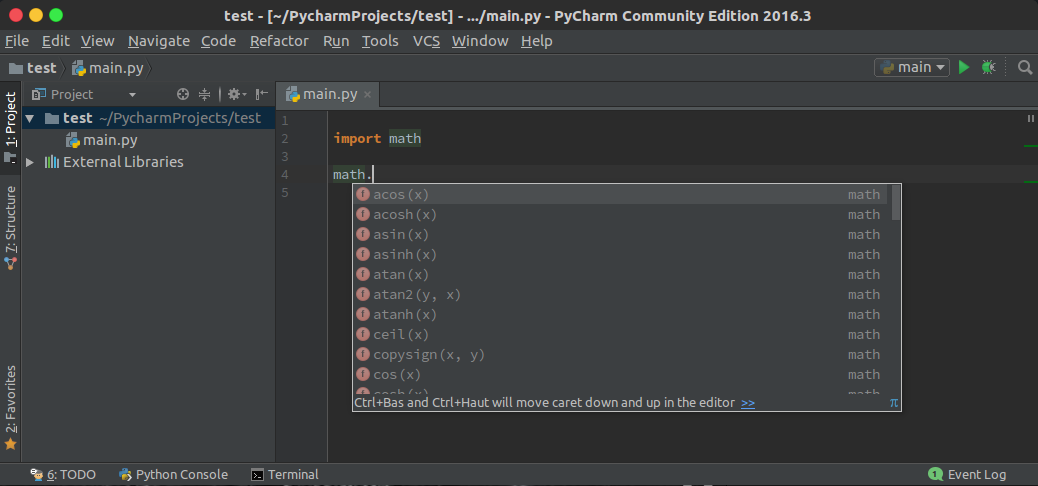
\includegraphics[width=\linewidth]{img/18_modules.png}
                \caption{La liste des fonctions du module math}
                \label{function_list}
            \end{figure}

            Vous pouvez parcourir cette liste avec les touches \code{bas} et \code{haut} pour voir toutes les fonctions
            contenu par ce module.

        \subsubsection{Le module random}
            Parmi les modules de python, on trouve le module \code{random}. Ce module nous permet de générer des
            nombres aléatoires.

            La fonction la plus intéressante de ce module est la fonction \code{randint()}. Cette fonction reçoit en
            paramètre deux entiers, et renvoie un nombre aléatoire entre ces deux entier. Voici un exemple
            d'utilisation :
            \begin{lstlisting}[style=code, breaklines=false]
import random

# la variable 'a' aura une valeur aléatoire compris entre
# 0 (inclut) et 100 (inclut)
a = random.randint(0, 100)

# la variable 'b' aura une valeur aléatoire compris entre
# -50 (inclut) et 300 (inclut)
b = random.randint(-50, 300)

print(a, b)
            \end{lstlisting}

            Vous pouvez vous amusez a re-exécuter ce code, et vous verrai qu'à chaque fois, les variables \code{a} et
            \code{b} prennent des valeurs différentes.

        \subsubsection{Quelles sont les modules disponibles ??}
            Python contient par défaut des centaines de modules, et comme c'est un langage très populaire et
            \emph{open source}, beaucoup de développeurs crée des modules très utiles et les partages avec la communauté.

            Parmi les modules crée par les développeurs, on trouve :
            \begin{itemize}
                \item Des modules pour d’interagir avec les bases de données,
                \item des modules pour faire de la programmation graphique,
                \item des modules pour afficher des barres de progressions,
                \item des modules pour manipuler les documents xml,
                \item \dots\ etc
            \end{itemize}

            On verra dans la fin de cette formation comment installer de nouveaux modules.

        \subsubsection{Exercice 7}
            Voici l'énoncé de l'exercice :
            \begin{itemize}
                \item Créez un projet nommé `exercice 7' et créez un fichier dedans nommé `main.py'.
                \item Chercher la fonction qui fait le factoriel dans le module \code{math}, et utiliser cette fonction
                    pour calculer le factoriel de \code{1000}.
            \end{itemize}
    \subsection{TP}
        Nous allons faire un TP qui regroupera tous les concepts que nous avons vu jusque là. Nous allons crée un
        mini jeu.

        Notre jeu va générer un nombre aléatoire, puis il va demander à l'utilisateur de trouver ce nombre. À chaque
        fois que l'utilisateur essaye de trouver ce nombre aléatoire, notre programme doit l'informer si c'est juste
        ou pas ; si ce n'est pas juste, notre programme doit dire à l'utilisateur si le nombre aléatoire est supérieur
        où inférieur au nombre donner par l'utilisateur.

        Voici un exemple du déroulement de notre programme :
        \begin{lstlisting}[style=exec_result]
J'ai générer un nombre aléatoire entre 0 et 100.
Trouve le nombre : 45
C'est plus
Trouve le nombre : 90
C'est moins
Trouve le nombre : 70
C'est moins
Trouve le nombre : 67
Bravo, vous avez trouvez le nombre que j'ai générer.
        \end{lstlisting}

        \subsubsection{La solution}

        \begin{lstlisting}[style=code, breaklines=false]
import random

nombre_aleatoire = random.randint(0, 100)
nombre_utilisateur = -1

print("J'ai générer un nombre aléatoire entre 0 et 100")

while nombre_utilisateur != nombre_aleatoire:
    nombre_utilisateur = input("Trouve le nombre : ")
    nombre_utilisateur = int(nombre_utilisateur)
    if nombre_aleatoire > nombre_utilisateur:
        print("C'est plus")
    elif nombre_aleatoire < nombre_utilisateur:
        print("C'est moins")
    elif nombre_aleatoire == nombre_utilisateur:
        print("Bravo, vous avez trouvez le nombre que j'ai générer.")
        \end{lstlisting}

        \subsubsection{Extension du programme}
            Maintenant que votre jeu est fonctionnel, mettez les instructions de votre programmes dans une fonction appelé
            \code{jouer}, et débrouiller vous pour que le jeux se répète si l'utilisateur a en vie de répéter.

            Voici un exemple du déroulement :
            \begin{lstlisting}[style=exec_result]
J'ai générer un nombre aléatoire entre 0 et 100.
Trouve le nombre : 45
C'est plus
Trouve le nombre : 90
C'est moins
Trouve le nombre : 70
C'est moins
Trouve le nombre : 67
Bravo, vous avez trouvez le nombre que j'ai générer.

Est-ce que vous voulez rejouer (o/n) : o

J'ai générer un nombre aléatoire entre 0 et 100.
Trouve le nombre : 55
C'est moins
.
.
.
        \end{lstlisting}

        \subsubsection{La solution}
        \begin{lstlisting}[style=code, breaklines=false]
import random


def jouer():

    nombre_aleatoire = random.randint(0, 100)
    nombre_utilisateur = -1

    print("J'ai générer un nombre aléatoire entre 0 et 100")

    while nombre_utilisateur != nombre_aleatoire:
        nombre_utilisateur = input("Trouve le nombre : ")
        nombre_utilisateur = int(nombre_utilisateur)
        if nombre_aleatoire > nombre_utilisateur:
            print("C'est plus")
        elif nombre_aleatoire < nombre_utilisateur:
            print("C'est moins")
        elif nombre_aleatoire == nombre_utilisateur:
            print("Bravo, vous avez trouvez le nombre que j'ai générer.")


# C'est à cette instruction que commence notre programme.
rejouer = ""
while rejouer != "n":
    jouer()
    rejouer = input("Est-ce que vous voulez rejouer (o/n)")
        \end{lstlisting}
    \subsection{Le help}
        Nous allons voir dans cette partie, comment faire pour obtenir de l'aide sur le fonctionnement d'une fonction
        ou d'un module.

        Disons par exemple que vous avez entendu parler que la fonction \code{print()} est utilisé pour l'affichage,
        mais le problème c'est que vous ne savez pas ce qu'elle fait exactement, ni comment l'utiliser. C'est là où
        le \code{help()} vient au secours.

        Le \code{help()} (qui signifie aide) est une fonction de python qui vous permet d'obtenir l'aide sur une
        fonction ou un module. On lui donne en paramètre le nom de la fonction où le module, et elle nous affiche
        qu'est-ce que fait ce dernier et comment l'utiliser.

        Continuons dans l'exemple de la fonction \code{print()}, écrivez et exécuter ce code dans PyCharm :
        \begin{lstlisting}[style=code]
help(print)
        \end{lstlisting}

        Ce qui vous affichera :
        \begin{lstlisting}[style=exec_result]
Help on built-in function print in module builtins:

print(...)
    print(value, ..., sep=' ', end='\n', file=sys.stdout, flush=False)

    Prints the values to a stream, or to sys.stdout by default.
    Optional keyword arguments:
    file:  a file-like object (stream); defaults to the current sys.stdout.
    sep:   string inserted between values, default a space.
    end:   string appended after the last value, default a newline.
    flush: whether to forcibly flush the stream.
        \end{lstlisting}

        On voit que la fonction \code{print()} peut être utilisé avec beaucoup d'option. Nous allons pas voir comment
        elle fonctionne exactement aujourd'hui, car on a pas assez d'information. Mais nous allons le voir plus tard si
        on aura le temps de terminer la formation.

        Continuons avec un autre exemple. Disons qu'on veut comprendre le module \code{math}, il suffit aussi d'appeler
        le \code{help()} comme on a fait avec la fonction \code{print()} :
        \begin{lstlisting}[style=code]
import math

help(math)
        \end{lstlisting}

        Voici une partie du résultat qui apparaît :
        \begin{lstlisting}[style=exec_result]
Help on built-in module math:

NAME
    math

DESCRIPTION
    This module is always available.  It provides access to the
    mathematical functions defined by the C standard.

FUNCTIONS
    acos(...)
        acos(x)

        Return the arc cosine (measured in radians) of x.

    acosh(...)
        acosh(x)

        Return the inverse hyperbolic cosine of x.
        \end{lstlisting}

        L'affichage est généralement divisé en 3 parties. La première partie est \code{NAME} qui est le nom du module ;
        la deuxième est \code{DESCRIPTION} qui est une bref description du contenu du module ; et la troisième partie
        est \code{FUNCTIONS} qui est l'ensemble de fonction contenu dans ce module. Vous remarquez aussi que
        chaque fonction est expliqué.

        Maintenant, supposons qu'on veut seulement connaître ce que fait la fonction \code{acos()}, et non pas tout
        le module math, comment fait on ?? Il suffit juste d'appeler le \code{help()} sur la fonction \code{acos()}
        seulement :
        \begin{lstlisting}[style=code]
import math

help(math.acos)
        \end{lstlisting}

        Ce qui nous affichera seulement l'aide de la fonction \code{acos()} du module \code{math} :
        \begin{lstlisting}[style=exec_result]
Help on built-in function acos in module math:

acos(...)
    acos(x)

    Return the arc cosine (measured in radians) of x.
        \end{lstlisting}

        Le \code{help()} est une fonctionnalité très importante, et elle vous sera très utile quand vous programmez.


\clearpage

\section{Les objets}
    \questionbox{Mais c'est quoi un objet déjà ??}

    Il n'y a pas une définition simple sur la notion d'objet, mais on peut le voir de cette manière : l'objet est
    comme une variable, mais il est beaucoup plus puissant et beaucoup plus pratique.

    Nous allons essayer de voir les différents types d'objets qui existes en python, et nous allons voir comment
    ils fonctionnent, et comment les utiliser. Ainsi nous allons comprendre de mieux en mieux la notion d'objet.

    \subsection{Les listes}
        Le premier objet que nous allons apprendre dans ce chapitre sont les listes.

        Une liste est un type objet qui peut contenir des objets ou des variables.

        Disons qu'on veut créer une listes des noms des gens qui participe à la formation, nous allons procédé de cette
        manière :
        \begin{lstlisting}[style=code]
participants = ["Amine", "Khaled", "Imene"]
        \end{lstlisting}

        Maintenant, on a un objet \code{participants} de type liste, qui contient les étudiants qui participe à la
        formation.

        Pour afficher notre objet de type liste, on utilise tout simplement \code{print()} :
        \begin{lstlisting}[style=code]
print(participants)
        \end{lstlisting}

        Et voici le résultat obtenu :
        \begin{lstlisting}[style=exec_result]
['Amine', 'Khaled', 'Imene']
        \end{lstlisting}

        On aurai pu mettre autant de personnes qu'on veut dans la liste,
        \subsubsection{Autres exemples}
            Nous allons créer quelques listes pour que vous comprenez.

            Une liste d'entiers :
            \begin{lstlisting}[style=code]
nombres = [10, 345, -46, 315]

print(nombres)
            \end{lstlisting}

            Une liste nombres décimaux :
            \begin{lstlisting}[style=code]
decimaux = [1.134, 100.3]

print(nombres)
            \end{lstlisting}

            Et voici le dernier exemple, une liste qui contient des variables et des objets de différents types :
            \begin{lstlisting}[style=code]
liste_heterogene = ["je suis une phrase", 13, 25, "salut", 22.5]

print(nombres)
            \end{lstlisting}
        \subsubsection{Accéder à un élément de la liste}
            Nous avons vu comment crée une liste et comment l'afficher en entière.

            \questionbox{Maintenant si on veut affiche juste un élément de la liste, comment va-t-on faire ?}

            Pour afficher un élément d'une liste, on utilise les \code{[]}. Par exemple, si on veut afficher le premier
            élément de notre liste des noms, on fait comme ça :
            \begin{lstlisting}[style=code]
participants = ["Amine", "Khaled", "Imene"]

print(participants[0])
            \end{lstlisting}

            Ceci nous affichera :
            \begin{lstlisting}[style=exec_result]
Amine
            \end{lstlisting}

            \cautionbox{Dans python, comme dans tous les langages de programmation qui se respectent, la numérotation
            des éléments commence de \code{0} et non pas de \code{1}. Donc le premier élément de la liste est situé à la
            position \code{0}, le 2ème élément à la position \code{1} \ldots}

            Donc le dernier élément de notre liste se situe à la position \code{2}, et on peut l'afficher de cette
            manière :
            \begin{lstlisting}[style=code]
print(participants[2])
            \end{lstlisting}

            Sachez qu'on peut aussi récupérer un élément de la liste et le stocker dans une variable en utilisant le
            \code{[]}. Exemple :
            \begin{lstlisting}[style=code]
participants = ["Amine", "Khaled", "Imene"]

un_element = participants[2]

# Ceci nous affichera Imene
print(un_element)
            \end{lstlisting}

        \subsubsection{Parcourir une liste}
            Pour parcourir une liste, on utilise la boucle \code{for} :
            \begin{lstlisting}[style=code]
participants = ["Amine", "Khaled", "Imene"]

for elm in participants:
    print("Nom :", elm)
            \end{lstlisting}

            À chaque itération de la boucle, \code{elm} prend le prochain élément de notre liste \code{participants}.
            Ainsi, le résultat de l'exécution c'est :
            \begin{lstlisting}[style=exec_result]
Nom : Amine
Nom : Khaled
Nom : Imene
            \end{lstlisting}

        \subsubsection{Exercice 8}
            Crée une liste qui contient ces éléments : \code{"Moustapha"}, \code{128}, \code{42.1}, \code{"Eau"},
            \code{"Tomate"}
            et parcourez cette liste avec la boucle \code{for}.


        \subsubsection{Opérations sur les listes}
            Nous allons voir maintenant la puissance des objets dont je vous ai parlé tout à l'heure.

            Chaque type d'objet a un ensemble d'opérations propre à lui, et qu'on peut utilisé directement.
            Le syntaxe pour utiliser une opération est le suivant :
            \begin{lstlisting}[style=code]
notre_objet.nom_operation()
            \end{lstlisting}

            Revenons à notre exemple. Disons que nous avons crée notre liste :
            \begin{lstlisting}[style=code]
participants = ["Amine", "Khaled", "Imene"]
            \end{lstlisting}

            Puis au milieu de notre programme, on veut ajouter un autre membre à notre liste de participants, comment
            allons nous faire ?? Et bien, il suffit tout simplement d'utiliser l'opération qui permet d'ajouter
            un nouveau élément à notre liste :
            \begin{lstlisting}[style=code]
participants.append("Hmidouche")
            \end{lstlisting}

            Ainsi, nous avons ajouté un autre membre à notre liste. Si vous afficher notre liste maintenant vous
            allez voir qu'elle contient un nouveau membre. Voici le code de notre programme :
            \begin{lstlisting}[style=code]
participants = ["Amine", "Khaled", "Imene"]
# Ceci nous affichera ["Amine", "Khaled", "Imene"]
print(participants)

participants.append("Hmidouche")
# Ceci nous affichera ["Amine", "Khaled", "Imene", "Hmidouche"]
print(participants)
            \end{lstlisting}


            Donnant un autre exemple d'une autre opération. Disons que maintenant, Amine s'est désinscrit de
            la formation, et on doit le supprimer de la liste. Pour cela, il suffit d'utiliser l'opération
            qui permet de supprimer un élément de la liste :
            \begin{lstlisting}[style=code]
participants.remove("Amine")
# Ceci nous affichera ["Khaled", "Imene", "Hmidouche"]
print(participants)
            \end{lstlisting}

            Pour chercher une opération dans un objet, on utilise la même technique qu'avec les modules. Il suffit
            juste d'écrire le nom de notre objet, suivi par un \code{.} , PyCharm alors nous affichera toutes les
            opérations qu'on peut utiliser sur cet objet.

        \subsubsection{Exercice 9}
            Crée la liste \code{participants} comme on a fait tout à l'heure, et chercher l'opération qui permet
            de trier cette liste. Quand vous la trouvez, triez la liste et affichez là.

        \subsubsection{Accéder au dernier élément de la liste}
            Pour accéder au dernier élément de notre liste, on peut utiliser la méthode standard : Celle de récuperer
            la taille de notre liste, puis accéder au dernier élément en utilisant cette taille :
            \begin{lstlisting}[style=code]
participants = ["Amine", "Khaled", "Imene"]
# On récupère la taille de notre liste dans la variable 'taille'
taille = len(participants)

# On affiche le dernier élément de notre liste
print(participants[taille - 1])
            \end{lstlisting}

            Ou on peut utiliser la méthode la plus approprié de python, qui est :
            \begin{lstlisting}[style=code]
participants = ["Amine", "Khaled", "Imene"]

# On affiche le dernier élément de notre liste
print(participants[-1])
            \end{lstlisting}

            Avec python, si on utilise des positions négatives, on accède aux éléments depuis la fin.
            Donc pour accéder au dernier élément on utilise \code{participants[-1]}, pour accéder à l'avant
            dernier élément, en utilise \code{participants[-2]} \ldots

    \subsection{Les string}
        Nous avons parlé sur les objets de types liste dans la parties précédentes, maintenant on va parler sur
        les objets de type \code{string}.

        Pour rappel, les objets de type \code{string} contiennent du texte. Exemple :
        \begin{lstlisting}[style=code]
phrase = "Salut tout le monde"
        \end{lstlisting}

        \notebox{Nous avons dit au début de la formation qu'on peut déclarer une variable qui contient
        du texte en utilisant les \code{""}. Mais sachez que ceux-ci
        ne sont pas des variables, mais plutôt des objets. J'ai dit que ce sont des variables pour vous aidez
        à comprendre seulement.}

        \subsubsection{Accéder à une lettre}
            Vous pouvez voir les strings comme une succession de lettres.
            Pour accéder aux lettres de notre \code{string}, on utilise les \code{[]} comme on a fait avec les listes :
            \begin{lstlisting}[style=code]
phrase = "Salut tout le monde"
# On récupère la première lettre
lettre1 = phrase[0]
# On récupère la 5ème lettre
lettre2 = phrase[5]
# On récupère la dernière lettre
lettre3 = phrase[-1]

print(lettre1, lettre2, lettre3)
            \end{lstlisting}

        \subsubsection{Des opérations sur les strings}
            Comme avec les liste, les objets de type \code{string} ont plusieurs opérations qu'on peut utiliser.

            Parmi ces opérations, on trouve l'opération qui vérifie si notre \code{string} contient que des lettres :
            \begin{lstlisting}[style=code]
phrase = "Salut tout le monde"
if phrase.isalpha():
    print("Notre string contient que des lettres.")
else :
    print("Non, il ne contient pas que des lettres.")
            \end{lstlisting}

            Il y a une autre opération qui vérifie si notre objet contient que des chiffres :
            \begin{lstlisting}[style=code]
telephone = "0550102030"
if telephone.isdigit():
    print("Notre string contient que des chiffres.")
else :
    print("Non, il ne contient pas que des chiffres.")
            \end{lstlisting}

            On trouve plusieurs opérations de ce genre qui font la vérification.
            Je vous donne deux autres si vous voulez les essayer à la maison :
            \begin{description}
                \item[isupper() :] Renvoie True si notre string contient que des majuscules.
                \item[islower() :] Renvoie True si notre string contient que des minuscules.
            \end{description}

        \subsubsection{Opérations avancées}
            Il existe une opération qui permet de chercher du texte dans notre string. C'est l'opération \code{find()} :
            \begin{lstlisting}[style=code]
phrase = "Salut tout le monde"
position = phrase.find("tout")

# Ceci nous affichera 6
print("Le mot 'tout' est au position", position)
            \end{lstlisting}

            L'opération \code{find} (celle qu'on vient de voir), nous renvoie la position du texte dans notre
            objet string. Si elle ne trouve pas le texte, alors elle nous renvoie la valeur \code{-1} .

            Allons voir une autre opérations très intéressantes. Disons qu'on veut diviser notre string en mot !
            Il suffit tout simplement d'utiliser l'opération \code{split()} comme ça :

            \begin{lstlisting}[style=code]
phrase = "Salut tout le monde"
# On demande que notre phrase soit diviser
# par rapport au espaces.
les_mots = phrase.split(" ")

# Ceci nous affichera : ["Salut", "tout", "le", "monde"]
print(les_mots)
            \end{lstlisting}

            L'opération \code{split()} divise notre string selon le séparateur qu'on lui a donnée en paramètre,
            et elle nous renvoie une liste contenant les éléments qu'elle a obtenu.

            Si on veut à nouveau joindre les éléments, il suffit d'utiliser l'opération \code{join()} :
            \begin{lstlisting}[style=code]
les_mots =  ["Salut", "tout", "le", "monde"]

# On demande que notre liste soit regroupé dans un string
# et que entre chaque éléments de la liste en met un espace
# ainsi on obtiendra a nouveau notre phrase.
une_autre_phrase = " ".join(les_mots)

# Ceci nous affichera : Salut tout le monde
print(une_autre_phrase)
            \end{lstlisting}

            \subsubsection{Exercice 10}
                Vous avez le string \code{"fromage,gâteau,tarte,pizza"}, diviser cette string en une liste selon le
                \code{,} ; puis joigne cette liste en utilisant le \code{-} pour à la fin obtenir
                \code{"fromage-gâteau-tarte-pizza"}.

        \subsection{Les dictionnaires}
%     \subsection{Les différents types d'objets disponible}
%         On parlera des string, listes, tuples et des dictionnaires.
%     \subsection{Les opérations sur les fichiers}
%         Ouverture, lecture, écriture des fichiers.
%     \subsection{Les chaînes de caractères}
%     \subsection{Les listes}
%     \subsection{Les tuples}
%     \subsection{Les dictionnaires}
%     \subsection{TP}

% \section{La programmation avancée}
%     \subsection{Exécutions des commandes systèmes}
%     \subsection{L'aléatoire}
%     \subsection{Gestion des mots de passes}
%     \subsection{Installer des modules python}

% \section{Allez plus loin}
%     Des tutos pour la programmation graphique avec PyQt. Le tuto d'openclassrooms.
\end{document}
